\section{数据库逻辑设计}\label{sec:LogicalDesign}

在本节(\cref{sec:LogicalDesign})中,我们将介绍数据库逻辑设计,包括数据库关系模式图、表设计、数据库设计和数据定义语言(DDL)设计。

\subsection{数据库关系模式图}

数据库关系模式图(\cref{fig:RelationshipSchema})的设计反映了本项目的信息系统。

\begin{figure}[htbp]
    \centering
    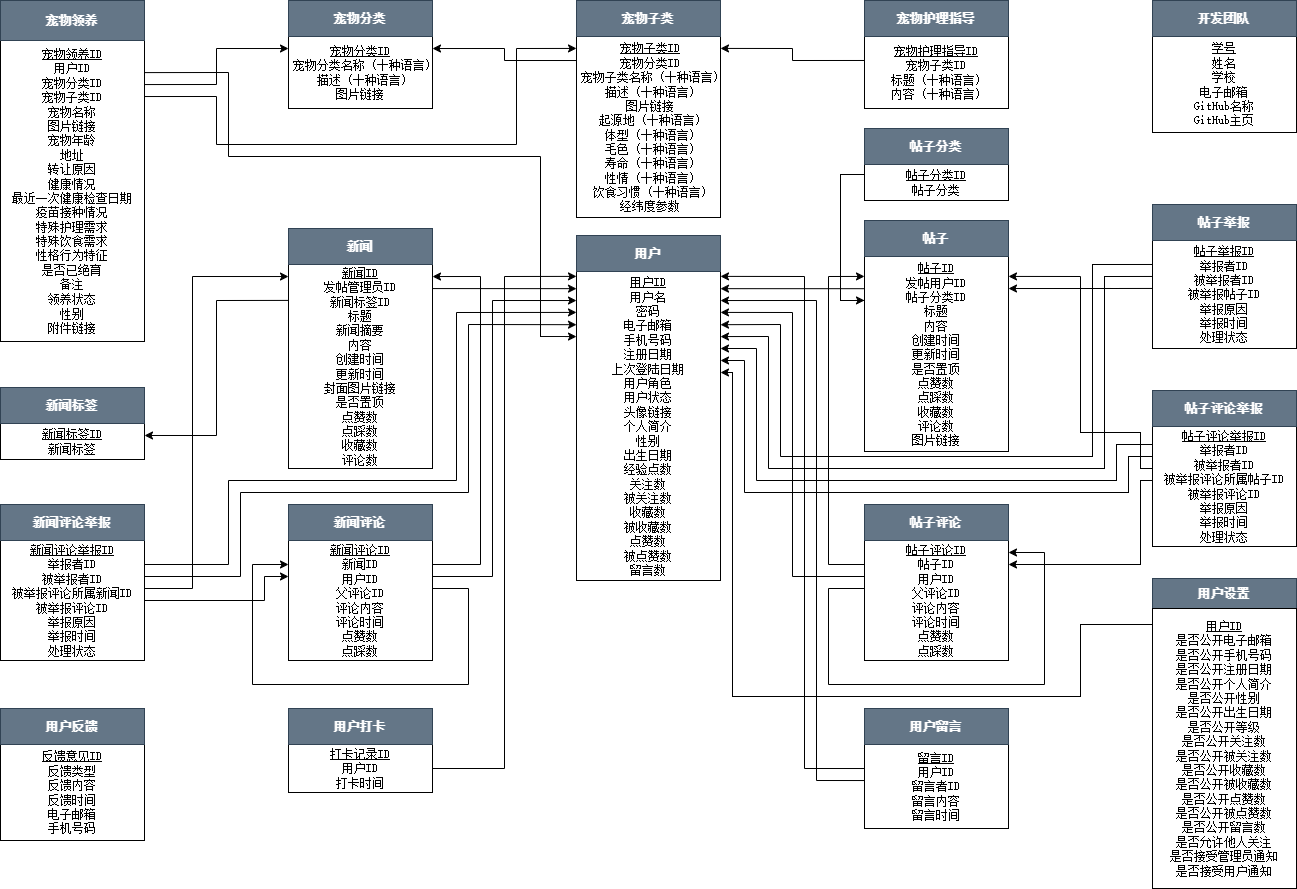
\includegraphics[width=\textwidth]{figures/RelationshipSchema.png}
    \caption{数据库关系模式图}
    \label{fig:RelationshipSchema}
\end{figure}

\subsubsection{模块化设计}

数据库的模块化设计通过将功能划分为独立的表来实现,例如用户信息、新闻、帖子和宠物等。每个模块作为一个单独的表存在,确保了系统内部的高度组织和结构化,同时显著降低了不同模块间的依赖性。

\subsubsection{用户中心设计}

用户表作为数据库中的核心表,通过“用户ID”与多个其他表如用户打卡表、用户留言表进行关联,这强调了用户在平台中的中心作用。该设计允许系统有效地集中处理和访问关于用户的所有信息,包括他们的个人设置、活动记录以及与其他用户的互动。这样的集中管理有助于优化用户体验,并确保数据的一致性和准确性。

\subsubsection{内容管理设计}

在内容管理方面,帖子表和新闻表是核心组件,与评论、点赞、点踩、收藏和举报等功能相关联。这种设计不仅体现了管理内容时的复杂性,还展示了如何有效追踪用户与内容的互动,如点赞和评论。此外,评论系统的设计支持对帖子和新闻的评论进行进一步的互动,如点赞或点踩,从而增强了平台的互动性和用户参与度。

\subsubsection{举报系统设计}

通过帖子举报表、帖子评论举报表和新闻评论举报表,本系统为用户提供了一个举报不当内容的有效机制。这些表的设计保证了用户可以安全地报告问题内容,同时系统能够有效地处理这些举报,确保平台内容的健康和合规性,维护了一个积极和健康的社区环境。

\subsubsection{宠物领养模块设计}

宠物领养模块通过宠物分类表、宠物子类表和宠物领养表的设计,实现了对宠物信息的详细分类和管理。这些表不仅提供了宠物的基本信息和分类,还详细记录了每只宠物的特定信息,如健康状况、领养需求等,确保潜在领养者能够找到与他们情况相匹配的宠物。

\subsubsection{开发团队信息设计}

开发团队表聚焦于记录平台维护和开发团队成员的详细信息,如姓名、联系方式、所属学校等。这不仅有助于内部的团队管理和沟通,也提供了一个渠道供用户了解开发团队的背景,从而增强用户对平台的信任和安全感。

\subsection{表设计}

在本项目中,我们设计了多种表来存储用户信息、社区互动、内容发布、新闻系统、宠物领养等信息,这些表设计体现了一个为宠物爱好者提供的一站式信息与资源交流天地的数据需求。

在表设计过程中,我们综合考虑了规范化、主键和索引、外键、数据类型和约束、安全性和隐私、性能优化、数据持久化、扩展性和可维护性等方面。这样的表设计涵盖了本平台的核心功能,但在实践中,可能需要根据实际应用场景和性能测试结果进行调整和优化,设计时也充分考虑了将来可能的功能扩展和数据迁移的便利性。

本项目设计的表及其属性如下:

\begin{enumerate}
    \item \textbf{用户表}(\underline{用户ID},用户名,密码,手机号码,注册日期,上次登录时间,用户角色,用户状态,头像链接,个人简介,性别,出生日期,经验点数,关注数,被关注数,收藏数,被收藏数,点赞数,被点赞数,留言数)
    \item \textbf{用户设置表}(\underline{用户ID},是否公开手机号码,是否公开注册日期,是否公开个人简介,是否公开性别,是否公开出生日期,是否公开等级,是否公开关注数,是否公开被关注数,是否公开收藏数,是否公开被收藏数,是否公开点赞数,是否公开被点赞数,是否公开留言数,是否允许他人关注,是否接受管理员通知,是否接受用户通知)
    \item \textbf{用户打卡表}(\underline{打卡记录ID},用户ID,打卡时间)
    \item \textbf{用户关注表}(\underline{被关注者ID},\underline{关注者ID},关注时间)
    \item \textbf{用户留言表}(\underline{留言ID},用户ID,留言者ID,留言内容,留言时间)
    \item \textbf{用户反馈表}(\underline{反馈意见ID},反馈类型,反馈内容,反馈时间,电子邮箱,手机号码)
    \item \textbf{帖子分类表}(\underline{帖子分类ID},帖子分类)
    \item \textbf{帖子表}(\underline{帖子ID},发帖用户ID,帖子分类ID,标题,内容,创建时间,更新时间,是否置顶,点赞数,点踩数,收藏数,评论数,图片链接)
    \item \textbf{帖子评论表}(\underline{帖子评论ID},帖子ID,用户ID,父评论ID,评论内容,评论时间,点赞数,点踩数)
    \item \textbf{帖子点赞表}(\underline{帖子ID},\underline{用户ID},点赞时间)
    \item \textbf{帖子点踩表}(\underline{帖子ID},\underline{用户ID},点踩时间)
    \item \textbf{帖子评论点赞表}(\underline{帖子评论ID},\underline{用户ID},点赞时间)
    \item \textbf{帖子评论点踩表}(\underline{帖子评论ID},\underline{用户ID},点踩时间)
    \item \textbf{帖子收藏表}(\underline{帖子ID},\underline{用户ID},收藏时间)
    \item \textbf{帖子举报表}(\underline{帖子举报ID},举报者ID,被举报者ID,被举报帖子ID,举报原因,举报时间,处理状态)
    \item \textbf{帖子评论举报表}(\underline{帖子评论举报ID},举报者ID,被举报者ID,被举报评论所属帖子ID,被举报评论ID,举报原因,举报时间,处理状态)
    \item \textbf{新闻标签表}(\underline{新闻标签ID},新闻标签)
    \item \textbf{新闻表}(\underline{新闻ID},管理员ID,新闻标签ID,标题,新闻摘要,内容,创建时间,更新时间,封面图片链接,是否置顶,点赞数,点踩数,收藏数,评论数)
    \item \textbf{新闻评论表}(\underline{新闻评论ID},新闻ID,用户ID,父评论ID,评论内容,评论时间,点赞数,点踩数)
    \item \textbf{新闻点赞表}(\underline{新闻ID},\underline{用户ID},点赞时间)
    \item \textbf{新闻点踩表}(\underline{新闻ID},\underline{用户ID},点踩时间)
    \item \textbf{新闻评论点赞表}(\underline{新闻评论ID},\underline{用户ID},点赞时间)
    \item \textbf{新闻评论点踩表}(\underline{新闻评论ID},\underline{用户ID},点踩时间)
    \item \textbf{新闻收藏表}(\underline{新闻ID},\underline{用户ID},收藏时间)
    \item \textbf{新闻评论举报表}(\underline{新闻评论举报ID},举报者ID,被举报者ID,被举报评论所属新闻ID,被举报评论ID,举报原因,举报时间,处理状态)
    \item \textbf{宠物分类表}(\underline{宠物分类ID},宠物分类名称(汉语),宠物分类名称(德语),宠物分类名称(英语),宠物分类名称(西班牙语),宠物分类名称(法语),宠物分类名称(意大利语),宠物分类名称(日语),宠物分类名称(韩语),宠物分类名称(葡萄牙语),宠物分类名称(俄语),描述(汉语),描述(德语),描述(英语),描述(西班牙语),描述(法语),描述(意大利语),描述(日语),描述(韩语),描述(葡萄牙语),描述(俄语),图片链接)
    \item \textbf{宠物子类表}(\underline{宠物子类ID},宠物分类ID,宠物子类名称(汉语),宠物子类名称(德语),宠物子类名称(英语),宠物子类名称(西班牙语),宠物子类名称(法语),宠物子类名称(意大利语),宠物子类名称(日语),宠物子类名称(韩语),宠物子类名称(葡萄牙语),宠物子类名称(俄语),描述(汉语),描述(德语),描述(英语),描述(西班牙语),描述(法语),描述(意大利语),描述(日语),描述(韩语),描述(葡萄牙语),描述(俄语),图片链接,起源地(汉语),起源地(德语),起源地(英语),起源地(西班牙语),起源地(法语),起源地(意大利语),起源地(日语),起源地(韩语),起源地(葡萄牙语),起源地(俄语),体型(汉语),体型(德语),体型(英语),体型(西班牙语),体型(法语),体型(意大利语),体型(日语),体型(韩语),体型(葡萄牙语),体型(俄语),毛色(汉语),毛色(德语),毛色(英语),毛色(西班牙语),毛色(法语),毛色(意大利语),毛色(日语),毛色(韩语),毛色(葡萄牙语),毛色(俄语),寿命(汉语),寿命(德语),寿命(英语),寿命(西班牙语),寿命(法语),寿命(意大利语),寿命(日语),寿命(韩语),寿命(葡萄牙语),寿命(俄语),性情(汉语),性情(德语),性情(英语),性情(西班牙语),性情(法语),性情(意大利语),性情(日语),性情(韩语),性情(葡萄牙语),性情(俄语),饮食习惯(汉语),饮食习惯(德语),饮食习惯(英语),饮食习惯(西班牙语),饮食习惯(法语),饮食习惯(意大利语),饮食习惯(日语),饮食习惯(韩语),饮食习惯(葡萄牙语),饮食习惯(俄语),经纬度参数)
    \item \textbf{宠物护理指导表}(\underline{宠物护理指导ID},宠物子类ID,标题(汉语),标题(德语),标题(英语),标题(西班牙语),标题(法语),标题(意大利语),标题(日语),标题(韩语),标题(葡萄牙语),标题(俄语),内容(汉语),内容(德语),内容(英语),内容(西班牙语),内容(法语),内容(意大利语),内容(日语),内容(韩语),内容(葡萄牙语),内容(俄语))
    \item \textbf{宠物领养表}(\underline{宠物领养ID},用户ID,宠物分类ID,宠物子类ID,宠物名称,图片链接,宠物年龄,地址,转让原因,健康情况,最近一次健康检查日期,疫苗接种情况,特殊护理需求,特殊饮食需求,性格行为特征,是否已绝育,备注,领养状态,性别,附件链接)
    \item \textbf{开发团队表}(\underline{学号},姓名,学校,电子邮箱,Github名称,Github主页)
\end{enumerate}

\subsubsection{用户表 USER}

用户表(USER)是社交平台数据库中核心的数据表之一,负责存储所有用户的基本信息和账户细节。该表包括了用户ID、用户名、密码、手机号码等标识性信息,以及用户的注册日期和最后登录时间等活动记录。此外,用户表还详细记录了用户的角色和状态,支持安全特性如密码保护。个人化数据如头像链接、个人简介、性别和出生日期也被包括在内,为用户提供个性化的服务。此表还记录了与用户活动相关的统计数据,如关注数、被关注数、收藏数、被收藏数、点赞数、被点赞数和留言数等,这些数据对于用户互动和平台运营分析尤为重要。整体上,用户表的设计旨在确保用户数据的完整性、安全性和高效的数据访问,以支持社交平台的日常运营和用户管理。(\cref{tab:UserTable})

\begin{longtable}[c]{@{}llrll@{}}
    \caption{用户表 USER}
    \label{tab:UserTable}                                                                       \\
    \toprule
    \textbf{字段名}       & \textbf{数据类型} & \textbf{长度} & \textbf{说明} & \textbf{备注}                \\ \midrule
    \endfirsthead
    \multicolumn{5}{r}{\textbf{续表~\thetable}}                                                   \\
    \toprule
    \textbf{字段名}       & \textbf{数据类型} & \textbf{长度} & \textbf{说明} & \textbf{备注}                \\ \midrule
    \endhead
    \hline
    \multicolumn{5}{r}{续下页}
    \endfoot
    \endlastfoot
    user\_id           & INT           &             & 用户 ID       & PK、非空                      \\
    user\_name         & VARCHAR       & 64          & 用户名         & 非空、唯一、最长存储16个中文字符          \\
    password           & VARCHAR       & 64          & 密码          & 非空、存储密码明文的哈希值              \\
    telephone          & VARCHAR       & 16          & 手机号码        & 非空、唯一                      \\
    registration\_date & DATE          &             & 注册日期        & 非空                         \\
    last\_login\_time  & DATE          &             & 上次登录时间      & 非空                         \\
    role               & NUMBER(1)     &             & 用户角色        & 非空、Boolean:0 - 普通用户;1 - 管理 \\
    status             & NUMBER(1)     &             & 用户状态        & 非空、Boolean:0 - 正常;1 - 封禁   \\
    avatar\_url        & VARCHAR       & 2048        & 头像链接        &                            \\
    profile            & VARCHAR       & 512         & 个人简介        & 最长存储128个中文字符               \\
    gender             & NUMBER(1)     &             & 性别          & 非空、Boolean:0 - 男性;1 - 女性   \\
    birthdate          & DATE          &             & 出生日期        & 非空                         \\
    experience\_points & INT           &             & 经验点数        & 非空                         \\
    follows\_count     & INT           &             & 关注数         & 非空                         \\
    followed\_count    & INT           &             & 被关注数        & 非空                         \\
    favorites\_count   & INT           &             & 收藏数         & 非空                         \\
    favorited\_count   & INT           &             & 被收藏数        & 非空                         \\
    likes\_count       & INT           &             & 点赞数         & 非空                         \\
    liked\_count       & INT           &             & 被点赞数        & 非空                         \\
    message\_count     & INT           &             & 留言数         & 非空                         \\ \bottomrule
\end{longtable}

\subsubsection{用户设置表 USER\_SETTING}

用户设置表(USER\_SETTING)是一个关键的数据表,用于存储和管理用户的个人偏好设置。这包括对隐私设置(例如是否公开邮箱、电话号码等个人信息)以及通知偏好(是否接收来自管理员或其他用户的通知)的选择。每个设置项都通过一个布尔字段来表示,确保用户可以个性化其在平台上的体验。表中的每一条记录都与用户表中的一个特定用户ID相关联,通过外键关系维护数据的一致性和完整性。(\cref{tab:UserSettingTable})

\begin{longtable}[c]{@{}llrll@{}}
    \caption{用户设置表 USER\_SETTING}
    \label{tab:UserSettingTable}                                                                            \\
    \toprule
    \textbf{字段名}                   & \textbf{数据类型} & \textbf{长度} & \textbf{说明} & \textbf{备注}                \\ \midrule
    \endfirsthead
    \multicolumn{5}{r}{\textbf{续表~\thetable}}                                                               \\
    \toprule
    \textbf{字段名}                   & \textbf{数据类型} & \textbf{长度} & \textbf{说明} & \textbf{备注}                \\ \midrule
    \endhead
    \hline
    \multicolumn{5}{r}{续下页}
    \endfoot
    \endlastfoot
    user\_id                       & INT           &             & 用户 ID       & PK、FK to USER(user\_id)、非空 \\
    is\_telephone\_public          & NUMBER(1)     &             & 是否公开手机号码    & 非空、Boolean:0 - 不公开;1 - 公开  \\
    is\_registration\_date\_public & NUMBER(1)     &             & 是否公开注册日期    & 非空、Boolean:0 - 不公开;1 - 公开  \\
    is\_profile\_public            & NUMBER(1)     &             & 是否公开个人简介    & 非空、Boolean:0 - 不公开;1 - 公开  \\
    is\_gender\_public             & NUMBER(1)     &             & 是否公开性别      & 非空、Boolean:0 - 不公开;1 - 公开  \\
    is\_birthdate\_public          & NUMBER(1)     &             & 是否公开出生日期    & 非空、Boolean:0 - 不公开;1 - 公开  \\
    is\_level\_public              & NUMBER(1)     &             & 是否公开等级      & 非空、Boolean:0 - 不公开;1 - 公开  \\
    is\_following\_count\_public   & NUMBER(1)     &             & 是否公开关注数     & 非空、Boolean:0 - 不公开;1 - 公开  \\
    is\_followers\_count\_public   & NUMBER(1)     &             & 是否公开被关注数    & 非空、Boolean:0 - 不公开;1 - 公开  \\
    is\_favorites\_count\_public   & NUMBER(1)     &             & 是否公开收藏数     & 非空、Boolean:0 - 不公开;1 - 公开  \\
    is\_favored\_count\_public     & NUMBER(1)     &             & 是否公开被收藏数    & 非空、Boolean:0 - 不公开;1 - 公开  \\
    is\_likes\_count\_public       & NUMBER(1)     &             & 是否公开点赞数     & 非空、Boolean:0 - 不公开;1 - 公开  \\
    is\_liked\_count\_public       & NUMBER(1)     &             & 是否公开被点赞数    & 非空、Boolean:0 - 不公开;1 - 公开  \\
    is\_message\_count\_public     & NUMBER(1)     &             & 是否公开留言数     & 非空、Boolean:0 - 不公开;1 - 公开  \\
    allow\_following               & NUMBER(1)     &             & 是否允许他人关注    & 非空、Boolean:0 - 不允许;1 - 允许  \\
    receive\_admin\_notifications  & NUMBER(1)     &             & 是否接受管理员通知   & 非空、Boolean:0 - 屏蔽;1 - 接受   \\
    receive\_user\_notifications   & NUMBER(1)     &             & 是否接受用户通知    & 非空、Boolean:0 - 屏蔽;1 - 接受   \\ \bottomrule
\end{longtable}

\subsubsection{用户打卡表 USER\_CHECK\_IN}

用户打卡表(USER\_CHECK\_IN)设计用来记录用户的每日打卡活动,支持用户习惯性的日常签到或特定任务的完成记录。该表包含三个主要字段:打卡记录ID(check\_in\_id),作为主键确保每条记录的唯一性;用户ID(user\_id),作为外键与用户表(USER)连接,表示哪个用户完成了打卡;以及打卡时间(check\_in\_time),记录用户具体的打卡时刻。此表的存在有助于促进用户的活跃参与和社交平台的用户粘性,同时为平台提供了一个简便的途径来跟踪和激励用户的日常活动。通过分析打卡数据,平台可以更好地了解用户活跃度,并根据这些数据优化用户体验和提供个性化的内容。(\cref{tab:UserCheckInTable})

\begin{longtable}[c]{@{}llrll@{}}
    \caption{用户打卡表 USER\_CHECK\_IN}
    \label{tab:UserCheckInTable}                                                          \\
    \toprule
    \textbf{字段名}    & \textbf{数据类型} & \textbf{长度} & \textbf{说明} & \textbf{备注}             \\ \midrule
    \endfirsthead
    \multicolumn{5}{r}{\textbf{续表~\thetable}}                                             \\
    \toprule
    \textbf{字段名}    & \textbf{数据类型} & \textbf{长度} & \textbf{说明} & \textbf{备注}             \\ \midrule
    \endhead
    \hline
    \multicolumn{5}{r}{续下页}
    \endfoot
    \endlastfoot
    check\_in\_id   & INT           &             & 打卡记录 ID     & PK、非空                   \\
    user\_id        & INT           &             & 用户 ID       & FK to USER(user\_id)、非空 \\
    check\_in\_time & DATE          &             & 打卡时间        & 非空                      \\ \bottomrule
\end{longtable}

\subsubsection{用户关注表 USER\_FOLLOW}

用户关注表(USER\_FOLLOW)是用于记录和管理用户之间关注关系的数据表。该表主要包含三个字段:被关注者ID(user\_id)、关注者ID(follower\_id)以及关注时间(follow\_time)。这两个ID字段均设为主键并与用户表(USER)的用户ID字段通过外键关联。(\cref{tab:UserFollowTable})

\begin{longtable}[c]{@{}llrll@{}}
    \caption{用户关注表 USER\_FOLLOW}
    \label{tab:UserFollowTable}                                                           \\
    \toprule
    \textbf{字段名} & \textbf{数据类型} & \textbf{长度} & \textbf{说明} & \textbf{备注}                \\ \midrule
    \endfirsthead
    \multicolumn{5}{r}{\textbf{续表~\thetable}}                                             \\
    \toprule
    \textbf{字段名} & \textbf{数据类型} & \textbf{长度} & \textbf{说明} & \textbf{备注}                \\ \midrule
    \endhead
    \hline
    \multicolumn{5}{r}{续下页}
    \endfoot
    \endlastfoot
    user\_id     & INT           &             & 被关注者 ID     & PK、FK to USER(user\_id)、非空 \\
    follower\_id & INT           &             & 关注者 ID      & PK、FK to USER(user\_id)、非空 \\
    follow\_time & DATE          &             & 关注时间        & 非空                         \\ \bottomrule
\end{longtable}

\subsubsection{用户留言表 USER\_MESSAGE}

用户留言表(USER\_MESSAGE)是设计用来记录用户间交流的留言信息的数据表。该表包含留言ID(message\_id),作为主键确保每条留言的唯一性;用户ID(user\_id)指被留言者,与用户表的用户ID通过外键关联;留言者ID(commenter\_id),也通过外键与用户表关联,表示留言的发送者;留言内容(message),存储用户之间传递的具体文本信息;以及留言时间(comment\_time),记录留言创建的具体时刻。(\cref{tab:UserMessageTable})

\begin{longtable}[c]{@{}llrll@{}}
    \caption{用户留言表 USER\_MESSAGE}
    \label{tab:UserMessageTable}                                                        \\
    \toprule
    \textbf{字段名}  & \textbf{数据类型} & \textbf{长度} & \textbf{说明} & \textbf{备注}             \\ \midrule
    \endfirsthead
    \multicolumn{5}{r}{\textbf{续表~\thetable}}                                           \\
    \toprule
    \textbf{字段名}  & \textbf{数据类型} & \textbf{长度} & \textbf{说明} & \textbf{备注}             \\ \midrule
    \endhead
    \hline
    \multicolumn{5}{r}{续下页}
    \endfoot
    \endlastfoot
    message\_id   & INT           &             & 留言 ID       & PK、非空                   \\
    user\_id      & INT           &             & 用户 ID       & FK to USER(user\_id)、非空 \\
    commenter\_id & INT           &             & 留言者 ID      & FK to USER(user\_id)、非空 \\
    message       & VARCHAR       & 512         & 留言内容        & 非空、最长存储128个中文字符         \\
    comment\_time & DATE          &             & 留言时间        & 非空                      \\ \bottomrule
\end{longtable}

\subsubsection{用户反馈表 USER\_FEEDBACK}

用户反馈表(USER\_FEEDBACK)用于记录和管理用户提供的反馈信息。该表包括多个字段,如反馈意见ID(feedback\_id),用作主键并且不能为空;反馈类型(feedback\_category)和反馈内容(feedback\_content),用以详细说明用户的反馈点,这两者均为必填项;反馈时间(feedback\_time),记录用户反馈的具体时间,也是必填项。此外,表中还包含用户的联系方式,如电子邮箱(email)和手机号码(telephone),这些字段可以为空,以便在需要时联系用户。整个表设计用于高效管理用户反馈,便于后续的分析和响应。(\cref{tab:UserFeedbackTable})

\begin{longtable}[c]{@{}llrll@{}}
    \caption{用户反馈表 USER\_FEEDBACK}
    \label{tab:UserFeedbackTable}                                                    \\
    \toprule
    \textbf{字段名}       & \textbf{数据类型} & \textbf{长度} & \textbf{说明} & \textbf{备注}     \\ \midrule
    \endfirsthead
    \multicolumn{5}{r}{\textbf{续表~\thetable}}                                        \\
    \toprule
    \textbf{字段名}       & \textbf{数据类型} & \textbf{长度} & \textbf{说明} & \textbf{备注}     \\ \midrule
    \endhead
    \hline
    \multicolumn{5}{r}{续下页}
    \endfoot
    \endlastfoot
    feedback\_id       & INT           &             & 反馈意见 ID     & PK、非空           \\
    feedback\_category & VARCHAR       & 32          & 反馈类型        & 非空              \\
    feedback\_content  & VARCHAR       & 2048        & 反馈内容        & 非空、最长存储512个中文字符 \\
    feedback\_time     & DATE          &             & 反馈时间        & 非空              \\
    email              & VARCHAR       & 2048        & 电子邮箱        &                 \\
    telephone          & VARCHAR       & 16          & 手机号码        &                 \\ \bottomrule
\end{longtable}

\subsubsection{帖子分类表 POST\_CATEGORY}

帖子分类表(POST\_CATEGORY)是是用来管理和组织社区中帖子的分类信息的重要数据结构。这个表的存在使得平台能够更有效地组织内容,用户可以根据分类快速找到自己感兴趣的帖子。同时,这种分类机制也便于平台进行内容的推荐和管理,通过分析不同分类下的用户行为和反馈,平台可以调整内容的发布和推广策略,以满足用户的不同需求。(\cref{tab:PostCategoryTable})

\begin{longtable}[c]{@{}llrll@{}}
    \caption{帖子分类表 POST\_CATEGORY}
    \label{tab:PostCategoryTable}                                                \\
    \toprule
    \textbf{字段名} & \textbf{数据类型} & \textbf{长度} & \textbf{说明} & \textbf{备注}       \\ \midrule
    \endfirsthead
    \multicolumn{5}{r}{\textbf{续表~\thetable}}                                    \\
    \toprule
    \textbf{字段名} & \textbf{数据类型} & \textbf{长度} & \textbf{说明} & \textbf{备注}       \\ \midrule
    \endhead
    \hline
    \multicolumn{5}{r}{续下页}
    \endfoot
    \endlastfoot
    category\_id & INT           &             & 帖子分类 ID     & PK、非空             \\
    category     & VARCHAR       & 64          & 帖子分类        & 非空、唯一、最长存储16个中文字符 \\ \bottomrule
\end{longtable}

\subsubsection{帖子表 POST}

帖子表(POST)是社交平台核心的数据结构,用于记录用户的发布内容。每条帖子包含唯一的帖子ID(post\_id)作为主键,关联的用户ID(user\_id)以链接到用户表,以及帖子的分类ID(category\_id)。帖子的主要信息包括标题(title)和内容(content),两者都有明确的字符长度限制。此外,帖子的生命周期通过创建时间(creation\_date)和更新时间(update\_date)进行跟踪。表中还包括一些用于社交互动的字段,如是否置顶(is\_sticky)、点赞数(like\_count)、点踩数(dislike\_count)、收藏数(favorite\_count)和评论数(comment\_count),以及可选的图片链接(image\_url)。这样的设计不仅优化了内容管理和用户互动,还提供了数据分析和内容推荐的基础。(\cref{tab:PostTable})

\begin{longtable}[c]{@{}llrll@{}}
    \caption{帖子表 POST}
    \label{tab:PostTable}                                                                               \\
    \toprule
    \textbf{字段名}    & \textbf{数据类型} & \textbf{长度} & \textbf{说明} & \textbf{备注}                           \\ \midrule
    \endfirsthead
    \multicolumn{5}{r}{\textbf{续表~\thetable}}                                                           \\
    \toprule
    \textbf{字段名}    & \textbf{数据类型} & \textbf{长度} & \textbf{说明} & \textbf{备注}                           \\ \midrule
    \endhead
    \hline
    \multicolumn{5}{r}{续下页}
    \endfoot
    \endlastfoot
    post\_id        & INT           &             & 帖子 ID       & PK、非空                                 \\
    user\_id        & INT           &             & 发帖用户 ID     & FK to USER(user\_id)、非空               \\
    category\_id    & INT           &             & 帖子分类 ID     & FK to POST\_CATEGORY(category\_id)、非空 \\
    title           & VARCHAR       & 256         & 标题          & 非空、最长存储64个中文字符                        \\
    content         & VARCHAR       & 2048        & 内容          & 非空、最长存储512个中文字符                       \\
    creation\_date  & DATE          &             & 创建时间        & 非空                                    \\
    update\_date    & DATE          &             & 更新时间        & 非空                                    \\
    is\_sticky      & NUMBER(1)     &             & 是否置顶        & 非空、Boolean:0 - 否;1 - 是                \\
    like\_count     & INT           &             & 点赞数         & 非空                                    \\
    dislike\_count  & INT           &             & 点踩数         & 非空                                    \\
    favorite\_count & INT           &             & 收藏数         & 非空                                    \\
    comment\_count  & INT           &             & 评论数         & 非空                                    \\
    image\_url      & VARCHAR       & 2048        & 图片链接        &                                       \\ \bottomrule
\end{longtable}

\subsubsection{帖子评论表 POST\_COMMENT}

帖子评论表(POST\_COMMENT)是设计用于存储用户对帖子的评论及其相互作用的数据表。此表包括多个字段,如评论ID(comment\_id),作为主键提供唯一标识;帖子ID(post\_id)和用户ID(user\_id),分别通过外键关联到帖子表(POST)和用户表(USER),确保评论与特定帖子和用户相关联;父评论ID(parent\_comment\_id),允许评论形成层级结构,增加对话的深度和复杂性。此外,该表还跟踪每条评论的点赞数(like\_count)和点踩数(dislike\_count),这些数据对于评估社区对评论的接受程度和互动活跃性非常重要。(\cref{tab:PostCommentTable})

\begin{longtable}[c]{@{}llrll@{}}
    \caption{帖子评论表 POST\_COMMENT}
    \label{tab:PostCommentTable}                                                                       \\
    \toprule
    \textbf{字段名}        & \textbf{数据类型} & \textbf{长度} & \textbf{说明} & \textbf{备注}                      \\ \midrule
    \endfirsthead
    \multicolumn{5}{r}{\textbf{续表~\thetable}}                                                          \\
    \toprule
    \textbf{字段名}        & \textbf{数据类型} & \textbf{长度} & \textbf{说明} & \textbf{备注}                      \\ \midrule
    \endhead
    \hline
    \multicolumn{5}{r}{续下页}
    \endfoot
    \endlastfoot
    comment\_id         & INT           &             & 帖子评论 ID     & PK、非空                            \\
    post\_id            & INT           &             & 帖子 ID       & FK to POST(post\_id)、非空          \\
    user\_id            & INT           &             & 用户 ID       & FK to USER(user\_id)、非空          \\
    parent\_comment\_id & INT           &             & 父评论 ID      & FK to POST\_COMMENT(comment\_id) \\
    content             & VARCHAR       & 512         & 评论内容        & 非空、最长存储128个中文字符                  \\
    comment\_time       & DATE          &             & 评论时间        & 非空                               \\
    like\_count         & INT           &             & 点赞数         & 非空                               \\
    dislike\_count      & INT           &             & 点踩数         & 非空                               \\ \bottomrule
\end{longtable}

\subsubsection{帖子点赞表 POST\_LIKE}

帖子点赞表(POST\_LIKE)是用于记录用户对帖子的点赞行为的数据表。该表主要包含三个字段:帖子ID(post\_id)和用户ID(user\_id),这两个字段都设置为主键,并通过外键分别与帖子表(POST)和用户表(USER)相关联,确保点赞的行为明确指向特定的帖子和用户;点赞时间(like\_time),记录用户进行点赞的具体时间。这种设计使得每个点赞都被独立记录,支持了对用户互动行为的详尽追踪,有助于增强内容的可见性和用户的参与感。此外,它也为社交平台提供了重要的数据,用于分析用户行为、优化内容推荐算法以及提升用户体验。(\cref{tab:PostLikeTable})

\begin{longtable}[c]{@{}llrll@{}}
    \caption{帖子点赞表 POST\_LIKE}
    \label{tab:PostLikeTable}                                                             \\
    \toprule
    \textbf{字段名} & \textbf{数据类型} & \textbf{长度} & \textbf{说明} & \textbf{备注}                \\ \midrule
    \endfirsthead
    \multicolumn{5}{r}{\textbf{续表~\thetable}}                                             \\
    \toprule
    \textbf{字段名} & \textbf{数据类型} & \textbf{长度} & \textbf{说明} & \textbf{备注}                \\ \midrule
    \endhead
    \hline
    \multicolumn{5}{r}{续下页}
    \endfoot
    \endlastfoot
    post\_id     & INT           &             & 帖子 ID       & PK、FK to POST(post\_id)、非空 \\
    user\_id     & INT           &             & 用户 ID       & PK、FK to USER(user\_id)、非空 \\
    like\_time   & DATE          &             & 点赞时间        & 非空                         \\ \bottomrule
\end{longtable}

\subsubsection{帖子点踩表 POST\_DISLIKE}

帖子点踩表(POST\_DISLIKE)是用于记录用户对帖子的不赞同或反对行为的数据表。该表主要包含三个字段:帖子ID(post\_id)和用户ID(user\_id),这两个字段均作为主键,并且分别通过外键与帖子表(POST)和用户表(USER)连接,确保点踩行为明确针对特定的帖子和特定的用户;点踩时间(dislike\_time),记录用户进行点踩的具体时刻。这种数据记录允许平台跟踪和分析不受欢迎或有争议的内容,为内容管理和质量控制提供参考。(\cref{tab:PostDislikeTable})

\begin{longtable}[c]{@{}llrll@{}}
    \caption{帖子点踩表 POST\_DISLIKE}
    \label{tab:PostDislikeTable}                                                           \\
    \toprule
    \textbf{字段名}  & \textbf{数据类型} & \textbf{长度} & \textbf{说明} & \textbf{备注}                \\ \midrule
    \endfirsthead
    \multicolumn{5}{r}{\textbf{续表~\thetable}}                                              \\
    \toprule
    \textbf{字段名}  & \textbf{数据类型} & \textbf{长度} & \textbf{说明} & \textbf{备注}                \\ \midrule
    \endhead
    \hline
    \multicolumn{5}{r}{续下页}
    \endfoot
    \endlastfoot
    post\_id      & INT           &             & 帖子 ID       & PK、FK to POST(post\_id)、非空 \\
    user\_id      & INT           &             & 用户 ID       & PK、FK to USER(user\_id)、非空 \\
    dislike\_time & DATE          &             & 点踩时间        & 非空                         \\ \bottomrule
\end{longtable}

\subsubsection{帖子评论点赞表 POST\_COMMENT\_LIKE}

帖子评论点赞表(POST\_COMMENT\_LIKE)是用于记录用户对帖子评论的赞同行为的数据表。该表包括三个主要字段:评论ID(comment\_id),用户ID(user\_id)和点赞时间(like\_time)。评论ID和用户ID共同作为复合主键,并通过外键分别与帖子评论表(POST\_COMMENT)和用户表(USER)关联,确保每个点赞行为都可以准确地链接到特定的评论和特定的用户。(\cref{tab:PostCommentLikeTable})

\begin{longtable}[c]{@{}llrll@{}}
    \caption{帖子评论点赞表 POST\_COMMENT\_LIKE}
    \label{tab:PostCommentLikeTable}                                                                  \\
    \toprule
    \textbf{字段名} & \textbf{数据类型} & \textbf{长度} & \textbf{说明} & \textbf{备注}                            \\ \midrule
    \endfirsthead
    \multicolumn{5}{r}{\textbf{续表~\thetable}}                                                         \\
    \toprule
    \textbf{字段名} & \textbf{数据类型} & \textbf{长度} & \textbf{说明} & \textbf{备注}                            \\ \midrule
    \endhead
    \hline
    \multicolumn{5}{r}{续下页}
    \endfoot
    \endlastfoot
    comment\_id  & INT           &             & 帖子评论 ID     & PK、FK to POST\_COMMENT(comment\_id)、非空 \\
    user\_id     & INT           &             & 用户 ID       & PK、FK to USER(user\_id)、非空             \\
    like\_time   & DATE          &             & 点赞时间        & 非空                                     \\ \bottomrule
\end{longtable}

\subsubsection{帖子评论点踩表 POST\_COMMENT\_DISLIKE}

帖子评论点踩表(POST\_COMMENT\_DISLIKE)是用于记录用户对帖子评论的不赞同或反对行为的数据表。该表的设计包括三个关键字段:评论ID(comment\_id)、用户ID(user\_id)和点踩时间(dislike\_time)。评论ID和用户ID共同构成复合主键,确保每条点踩记录都是独一无二的,并通过外键与帖子评论表(POST\_COMMENT)及用户表(USER)相连接,从而确保每个点踩行为都能准确指向特定的评论和特定的用户。点踩时间字段记录了点踩的具体时刻。这种记录机制不仅帮助平台监控社区内的负面互动,也提供了反馈机制,用于评估内容的争议性,支持平台在必要时采取相应的内容管理措施以维护健康的讨论环境。(\cref{tab:PostCommentDislikeTable})

\begin{longtable}[c]{@{}llrll@{}}
    \caption{帖子评论点踩表 POST\_COMMENT\_DISLIKE}
    \label{tab:PostCommentDislikeTable}                                                                \\
    \toprule
    \textbf{字段名}  & \textbf{数据类型} & \textbf{长度} & \textbf{说明} & \textbf{备注}                            \\ \midrule
    \endfirsthead
    \multicolumn{5}{r}{\textbf{续表~\thetable}}                                                          \\
    \toprule
    \textbf{字段名}  & \textbf{数据类型} & \textbf{长度} & \textbf{说明} & \textbf{备注}                            \\ \midrule
    \endhead
    \hline
    \multicolumn{5}{r}{续下页}
    \endfoot
    \endlastfoot
    comment\_id   & INT           &             & 帖子评论 ID     & PK、FK to POST\_COMMENT(comment\_id)、非空 \\
    user\_id      & INT           &             & 用户 ID       & PK、FK to USER(user\_id)、非空             \\
    dislike\_time & DATE          &             & 点踩时间        & 非空                                     \\ \bottomrule
\end{longtable}

\subsubsection{帖子收藏表 POST\_FAVORITE}

帖子收藏表(POST\_FAVORITE)是设计用来记录用户对帖子的收藏行为的数据表,使用户能够保存他们喜欢或希望稍后查看的内容。此表包含三个主要字段:帖子ID(post\_id)、用户ID(user\_id)和收藏时间(favorite\_time)。帖子ID和用户ID共同作为复合主键,并通过外键分别与帖子表(POST)和用户表(USER)关联,确保每次收藏都能准确地指向特定的帖子和用户。收藏时间字段记录了用户收藏帖子的具体时间点。此表的存在不仅方便用户管理他们感兴趣的内容,也为平台提供了关于用户喜好和内容受欢迎程度的重要数据,有助于优化内容推荐算法和提高用户满意度。(\cref{tab:PostFavoriteTable})

\begin{longtable}[c]{@{}llrll@{}}
    \caption{帖子收藏表 POST\_FAVORITE}
    \label{tab:PostFavoriteTable}                                                           \\
    \toprule
    \textbf{字段名}   & \textbf{数据类型} & \textbf{长度} & \textbf{说明} & \textbf{备注}                \\ \midrule
    \endfirsthead
    \multicolumn{5}{r}{\textbf{续表~\thetable}}                                               \\
    \toprule
    \textbf{字段名}   & \textbf{数据类型} & \textbf{长度} & \textbf{说明} & \textbf{备注}                \\ \midrule
    \endhead
    \hline
    \multicolumn{5}{r}{续下页}
    \endfoot
    \endlastfoot
    post\_id       & INT           &             & 帖子 ID       & PK、FK to POST(post\_id)、非空 \\
    user\_id       & INT           &             & 用户 ID       & PK、FK to USER(user\_id)、非空 \\
    favorite\_time & DATE          &             & 收藏时间        & 非空                         \\ \bottomrule
\end{longtable}

\subsubsection{帖子举报表 POST\_REPORT}

帖子举报表(POST\_REPORT)是用于记录用户对不适当或违反社区规定的帖子的举报行为的数据表。该表具备举报的详细信息,包括举报ID(post\_report\_id),作为主键确保每条举报记录的唯一性;举报者ID(reporter\_id)和被举报者ID(reported\_user\_id),通过外键与用户表(USER)关联,明确举报与被举报的用户;被举报帖子ID(reported\_post\_id),通过外键与帖子表(POST)关联,指向具体的被举报内容。此外,举报原因(report\_reason)详细记录用户举报的具体理由,举报时间(report\_time)记录了举报发生的具体时刻,处理状态(status)跟踪举报的审查进度。(\cref{tab:PostReportTable})

\begin{longtable}[c]{@{}llrll@{}}
    \caption{帖子举报表 POST\_REPORT}
    \label{tab:PostReportTable}                                                                 \\
    \toprule
    \textbf{字段名}       & \textbf{数据类型} & \textbf{长度} & \textbf{说明} & \textbf{备注}                \\ \midrule
    \endfirsthead
    \multicolumn{5}{r}{\textbf{续表~\thetable}}                                                   \\
    \toprule
    \textbf{字段名}       & \textbf{数据类型} & \textbf{长度} & \textbf{说明} & \textbf{备注}                \\ \midrule
    \endhead
    \hline
    \multicolumn{5}{r}{续下页}
    \endfoot
    \endlastfoot
    post\_report\_id   & INT           &             & 帖子举报 ID     & PK、非空                      \\
    reporter\_id       & INT           &             & 举报者 ID      & FK to USER(user\_id)、非空    \\
    reported\_user\_id & INT           &             & 被举报者 ID     & FK to USER(user\_id)、非空    \\
    reported\_post\_id & INT           &             & 被举报帖子 ID    & FK to POST(post\_id)、非空    \\
    report\_reason     & VARCHAR       & 512         & 举报原因        & 非空、最长存储128个中文字符            \\
    report\_time       & DATE          &             & 举报时间        & 非空                         \\
    status             & NUMBER(1)     &             & 处理状态        & 非空、Boolean:0 - 待处理;1 - 已处理 \\ \bottomrule
\end{longtable}

\subsubsection{帖子评论举报表 POST\_COMMENT\_REPORT}

帖子评论举报表(POST\_COMMENT\_REPORT)旨在记录用户对帖子评论的举报情况,特别是针对违规或不当评论的反馈。该表包括举报ID(post\_comment\_report\_id)作为主键,以确保每条举报记录的唯一性;举报者ID(reporter\_id)和被举报者ID(reported\_user\_id),通过外键与用户表(USER)关联,明确指明举报和被举报的用户身份;被举报评论所属帖子ID(reported\_post\_id)和被举报评论ID(reported\_comment\_id),通过外键与帖子表(POST)和帖子评论表(POST\_COMMENT)关联,精确指向被举报的具体评论。(\cref{tab:PostCommentReportTable})

\begin{longtable}[c]{@{}llrll@{}}
    \caption{帖子评论举报表 POST\_COMMENT\_REPORT}
    \label{tab:PostCommentReportTable}                                                                           \\
    \toprule
    \textbf{字段名}              & \textbf{数据类型} & \textbf{长度} & \textbf{说明}  & \textbf{备注}                         \\ \midrule
    \endfirsthead
    \multicolumn{5}{r}{\textbf{续表~\thetable}}                                                                    \\
    \toprule
    \textbf{字段名}              & \textbf{数据类型} & \textbf{长度} & \textbf{说明}  & \textbf{备注}                         \\ \midrule
    \endhead
    \hline
    \multicolumn{5}{r}{续下页}
    \endfoot
    \endlastfoot
    post\_comment\_report\_id & INT           &             & 帖子评论举报 ID    & PK、非空                               \\
    reporter\_id              & INT           &             & 举报者 ID       & FK to USER(user\_id)、非空             \\
    reported\_user\_id        & INT           &             & 被举报者 ID      & FK to USER(user\_id)、非空             \\
    reported\_post\_id        & INT           &             & 被举报评论所属帖子 ID & FK to POST(post\_id)、非空             \\
    reported\_comment\_id     & INT           &             & 被举报评论 ID     & FK to POST\_COMMENT(comment\_id)、非空 \\
    report\_reason            & VARCHAR       & 512         & 举报原因         & 非空、最长存储128个中文字符                     \\
    report\_time              & DATE          &             & 举报时间         & 非空                                  \\
    status                    & NUMBER(1)     &             & 处理状态         & 非空、Boolean:0 - 待处理;1 - 已处理          \\ \bottomrule
\end{longtable}

\subsubsection{新闻标签表 NEWS\_TAG}

新闻标签表(NEWS\_TAG)是用来管理和分类新闻内容的关键数据表,它通过标签系统来组织新闻文章,便于用户浏览和搜索特定主题的新闻。该表包含两个主要字段:新闻标签ID(tag\_id),作为主键确保每个标签的唯一性;以及新闻标签(tag),存储标签的文本描述,这是一个简短的字符字段,用于标记新闻内容的主题或类别。此字段设置为唯一,确保不会有重复的标签存在。通过这种方式,新闻标签表支持新闻管理系统的高效运作,使得新闻内容能够按照特定的主题或兴趣点被有效地分类和检索,增强了用户体验并提高了内容的可访问性。(\cref{tab:NewsTagTable})

\begin{longtable}[c]{@{}llrll@{}}
    \caption{新闻标签表 NEWS\_TAG}
    \label{tab:NewsTagTable}                                                     \\
    \toprule
    \textbf{字段名} & \textbf{数据类型} & \textbf{长度} & \textbf{说明} & \textbf{备注}       \\ \midrule
    \endfirsthead
    \multicolumn{5}{r}{\textbf{续表~\thetable}}                                    \\
    \toprule
    \textbf{字段名} & \textbf{数据类型} & \textbf{长度} & \textbf{说明} & \textbf{备注}       \\ \midrule
    \endhead
    \hline
    \multicolumn{5}{r}{续下页}
    \endfoot
    \endlastfoot
    tag\_id      & INT           &             & 新闻标签 ID     & PK、非空             \\
    tag          & VARCHAR       & 64          & 新闻标签        & 非空、唯一、最长存储16个中文字符 \\ \bottomrule
\end{longtable}

\subsubsection{新闻表 NEWS}

新闻表(NEWS)是设计用来存储和管理社交平台上发布的新闻内容的数据表。此表包括新闻ID(news\_id),作为主键确保每篇新闻的唯一性;管理员ID(user\_id),通过外键与用户表(USER)连接,标识新闻的发布者;新闻标签ID(tag\_id),通过外键与新闻标签表(NEWS\_TAG)连接,归类新闻主题。新闻的基本属性如标题(title)、摘要(summary)、详细内容(content)、创建和更新时间,以及封面图片链接(cover\_url)都被记录在表中。(\cref{tab:NewsTable})

\begin{longtable}[c]{@{}llrll@{}}
    \caption{新闻表 NEWS}
    \label{tab:NewsTable}                                                                     \\
    \toprule
    \textbf{字段名}    & \textbf{数据类型} & \textbf{长度} & \textbf{说明} & \textbf{备注}                 \\ \midrule
    \endfirsthead
    \multicolumn{5}{r}{\textbf{续表~\thetable}}                                                 \\
    \toprule
    \textbf{字段名}    & \textbf{数据类型} & \textbf{长度} & \textbf{说明} & \textbf{备注}                 \\ \midrule
    \endhead
    \hline
    \multicolumn{5}{r}{续下页}
    \endfoot
    \endlastfoot
    news\_id        & INT           &             & 新闻 ID       & PK、非空                       \\
    user\_id        & INT           &             & 管理员 ID      & FK to USER(user\_id)、非空     \\
    tag\_id         & INT           &             & 新闻标签 ID     & FK to NEWS\_TAG(tag\_id)、非空 \\
    title           & VARCHAR       & 256         & 标题          & 非空、最长存储64个中文字符              \\
    summary         & VARCHAR       & 512         & 新闻摘要        & 非空、最长存储128个中文字符             \\
    content         & CLOB          &             & 内容          & 非空                          \\
    creation\_date  & DATE          &             & 创建时间        & 非空                          \\
    update\_date    & DATE          &             & 更新时间        & 非空                          \\
    cover\_url      & VARCHAR       & 2048        & 封面图片链接      & 非空                          \\
    is\_sticky      & NUMBER(1)     &             & 是否置顶        & 非空、Boolean:0 - 否;1 - 是      \\
    like\_count     & INT           &             & 点赞数         & 非空                          \\
    dislike\_count  & INT           &             & 点踩数         & 非空                          \\
    favorite\_count & INT           &             & 收藏数         & 非空                          \\
    comment\_count  & INT           &             & 评论数         & 非空                          \\ \bottomrule
\end{longtable}

\subsubsection{新闻评论表 NEWS\_COMMENT}

新闻评论表(NEWS\_COMMENT)是设计用来存储用户对新闻文章的评论及其相关互动的数据表。此表包括多个字段,其中新闻评论ID(comment\_id)作为主键确保每条评论的唯一性;新闻ID(news\_id)和用户ID(user\_id)分别通过外键与新闻表(NEWS)和用户表(USER)关联,指明评论针对的具体新闻和发表评论的用户;父评论ID(parent\_comment\_id)允许评论具有层级结构,即回复其他评论。(\cref{tab:NewsCommentTable})

\begin{longtable}[c]{@{}llrll@{}}
    \caption{新闻评论表 NEWS\_COMMENT}
    \label{tab:NewsCommentTable}                                                                       \\
    \toprule
    \textbf{字段名}        & \textbf{数据类型} & \textbf{长度} & \textbf{说明} & \textbf{备注}                      \\ \midrule
    \endfirsthead
    \multicolumn{5}{r}{\textbf{续表~\thetable}}                                                          \\
    \toprule
    \textbf{字段名}        & \textbf{数据类型} & \textbf{长度} & \textbf{说明} & \textbf{备注}                      \\ \midrule
    \endhead
    \hline
    \multicolumn{5}{r}{续下页}
    \endfoot
    \endlastfoot
    comment\_id         & INT           &             & 新闻评论 ID     & PK、非空                            \\
    news\_id            & INT           &             & 新闻 ID       & FK to NEWS(news\_id)、非空          \\
    user\_id            & INT           &             & 用户 ID       & FK to USER(user\_id)、非空          \\
    parent\_comment\_id & INT           &             & 父评论 ID      & FK to NEWS\_COMMENT(comment\_id) \\
    content             & VARCHAR       & 512         & 评论内容        & 非空、最长存储128个中文字符                  \\
    comment\_time       & DATE          &             & 评论时间        & 非空                               \\
    like\_count         & INT           &             & 点赞数         & 非空                               \\
    dislike\_count      & INT           &             & 点踩数         & 非空                               \\ \bottomrule
\end{longtable}

\subsubsection{新闻点赞表 NEWS\_LIKE}

新闻点赞表(NEWS\_LIKE)是用来记录用户对新闻内容表达赞同或支持的行为的数据表。该表包含三个主要字段:新闻ID(news\_id)、用户ID(user\_id)和点赞时间(like\_time)。新闻ID和用户ID共同作为复合主键,并且通过外键分别与新闻表(NEWS)和用户表(USER)关联,这确保了每个点赞行为都能精确地关联到特定的新闻和特定的用户。点赞时间字段记录了用户进行点赞的具体时刻。这种记录机制有助于增强新闻互动性,同时帮助平台优化内容推送。(\cref{tab:NewsLikeTable})

\begin{longtable}[c]{@{}llrll@{}}
    \caption{新闻点赞表 NEWS\_LIKE}
    \label{tab:NewsLikeTable}                                                             \\
    \toprule
    \textbf{字段名} & \textbf{数据类型} & \textbf{长度} & \textbf{说明} & \textbf{备注}                \\ \midrule
    \endfirsthead
    \multicolumn{5}{r}{\textbf{续表~\thetable}}                                             \\
    \toprule
    \textbf{字段名} & \textbf{数据类型} & \textbf{长度} & \textbf{说明} & \textbf{备注}                \\ \midrule
    \endhead
    \hline
    \multicolumn{5}{r}{续下页}
    \endfoot
    \endlastfoot
    news\_id     & INT           &             & 新闻 ID       & PK、FK to NEWS(news\_id)、非空 \\
    user\_id     & INT           &             & 用户 ID       & PK、FK to USER(user\_id)、非空 \\
    like\_time   & DATE          &             & 点赞时间        & 非空                         \\ \bottomrule
\end{longtable}

\subsubsection{新闻点踩表 NEWS\_DISLIKE}

新闻点踩表(NEWS\_DISLIKE)用于记录用户对新闻内容的不赞同或反对的行为。这张表包含三个主要字段:新闻ID(news\_id)、用户ID(user\_id)和点踩时间(dislike\_time)。新闻ID和用户ID作为复合主键,并通过外键与新闻表(NEWS)和用户表(USER)关联,确保每个点踩行为都与特定的新闻和用户直接关联。点踩时间字段记录了用户进行点踩的具体时刻。(\cref{tab:NewsDislikeTable})

\begin{longtable}[c]{@{}llrll@{}}
    \caption{新闻点踩表 NEWS\_DISLIKE}
    \label{tab:NewsDislikeTable}                                                           \\
    \toprule
    \textbf{字段名}  & \textbf{数据类型} & \textbf{长度} & \textbf{说明} & \textbf{备注}                \\ \midrule
    \endfirsthead
    \multicolumn{5}{r}{\textbf{续表~\thetable}}                                              \\
    \toprule
    \textbf{字段名}  & \textbf{数据类型} & \textbf{长度} & \textbf{说明} & \textbf{备注}                \\ \midrule
    \endhead
    \hline
    \multicolumn{5}{r}{续下页}
    \endfoot
    \endlastfoot
    news\_id      & INT           &             & 新闻 ID       & PK、FK to NEWS(news\_id)、非空 \\
    user\_id      & INT           &             & 用户 ID       & PK、FK to USER(user\_id)、非空 \\
    dislike\_time & DATE          &             & 点踩时间        & 非空                         \\ \bottomrule
\end{longtable}

\subsubsection{新闻评论点赞表 NEWS\_COMMENT\_LIKE}

新闻评论点赞表(NEWS\_COMMENT\_LIKE)是专门用于记录用户对新闻评论的赞同行为的数据表。此表包含三个核心字段:评论ID(comment\_id)、用户ID(user\_id)、和点赞时间(like\_time)。评论ID和用户ID共同作为复合主键,与新闻评论表(NEWS\_COMMENT)和用户表(USER)关联。(\cref{tab:NewsCommentLikeTable})

\begin{longtable}[c]{@{}llrll@{}}
    \caption{新闻评论点赞表 NEWS\_COMMENT\_LIKE}
    \label{tab:NewsCommentLikeTable}                                                                  \\
    \toprule
    \textbf{字段名} & \textbf{数据类型} & \textbf{长度} & \textbf{说明} & \textbf{备注}                            \\ \midrule
    \endfirsthead
    \multicolumn{5}{r}{\textbf{续表~\thetable}}                                                         \\
    \toprule
    \textbf{字段名} & \textbf{数据类型} & \textbf{长度} & \textbf{说明} & \textbf{备注}                            \\ \midrule
    \endhead
    \hline
    \multicolumn{5}{r}{续下页}
    \endfoot
    \endlastfoot
    comment\_id  & INT           &             & 新闻评论 ID     & PK、FK to NEWS\_COMMENT(comment\_id)、非空 \\
    user\_id     & INT           &             & 用户 ID       & PK、FK to USER(user\_id)、非空             \\
    like\_time   & DATE          &             & 点赞时间        & 非空                                     \\ \bottomrule
\end{longtable}

\subsubsection{新闻评论点踩表 NEWS\_COMMENT\_DISLIKE}

新闻评论点踩表(NEWS\_COMMENT\_DISLIKE)旨在记录用户对新闻评论的不赞同或反对行为的详细数据。该表包含三个主要字段:评论ID(comment\_id)、用户ID(user\_id)和点踩时间(dislike\_time)。评论ID和用户ID作为复合主键,并且通过外键分别与新闻评论表(NEWS\_COMMENT)和用户表(USER)关联,确保每条点踩记录准确关联到特定的评论和用户。(\cref{tab:NewsCommentDislikeTable})

\begin{longtable}[c]{@{}llrll@{}}
    \caption{新闻评论点踩表 NEWS\_COMMENT\_DISLIKE}
    \label{tab:NewsCommentDislikeTable}                                                                \\
    \toprule
    \textbf{字段名}  & \textbf{数据类型} & \textbf{长度} & \textbf{说明} & \textbf{备注}                            \\ \midrule
    \endfirsthead
    \multicolumn{5}{r}{\textbf{续表~\thetable}}                                                          \\
    \toprule
    \textbf{字段名}  & \textbf{数据类型} & \textbf{长度} & \textbf{说明} & \textbf{备注}                            \\ \midrule
    \endhead
    \hline
    \multicolumn{5}{r}{续下页}
    \endfoot
    \endlastfoot
    comment\_id   & INT           &             & 新闻评论 ID     & PK、FK to NEWS\_COMMENT(comment\_id)、非空 \\
    user\_id      & INT           &             & 用户 ID       & PK、FK to USER(user\_id)、非空             \\
    dislike\_time & DATE          &             & 点踩时间        & 非空                                     \\ \bottomrule
\end{longtable}

\subsubsection{新闻收藏表 NEWS\_FAVORITE}

新闻收藏表(NEWS\_FAVORITE)是设计用来记录用户对新闻文章的收藏行为的数据表。该表使用户能够保存他们感兴趣的新闻内容以便未来查阅。包含三个主要字段:新闻ID(news\_id)和用户ID(user\_id),这两者共同构成复合主键并通过外键分别与新闻表(NEWS)和用户表(USER)连接;收藏时间(favorite\_time)记录了用户收藏新闻的具体时刻。(\cref{tab:NewsFavoriteTable})

\begin{longtable}[c]{@{}llrll@{}}
    \caption{新闻收藏表 NEWS\_FAVORITE}
    \label{tab:NewsFavoriteTable}                                                           \\
    \toprule
    \textbf{字段名}   & \textbf{数据类型} & \textbf{长度} & \textbf{说明} & \textbf{备注}                \\ \midrule
    \endfirsthead
    \multicolumn{5}{r}{\textbf{续表~\thetable}}                                               \\
    \toprule
    \textbf{字段名}   & \textbf{数据类型} & \textbf{长度} & \textbf{说明} & \textbf{备注}                \\ \midrule
    \endhead
    \hline
    \multicolumn{5}{r}{续下页}
    \endfoot
    \endlastfoot
    news\_id       & INT           &             & 新闻 ID       & PK、FK to NEWS(news\_id)、非空 \\
    user\_id       & INT           &             & 用户 ID       & PK、FK to USER(user\_id)、非空 \\
    favorite\_time & DATE          &             & 收藏时间        & 非空                         \\ \bottomrule
\end{longtable}

\subsubsection{新闻评论举报表 NEWS\_COMMENT\_REPORT}

新闻评论举报表(NEWS\_COMMENT\_REPORT)用于记录用户对不当或不适宜的新闻评论的举报行为。该表的设计包含多个字段,主要包括新闻评论举报ID(news\_comment\_report\_id)作为主键,确保每条举报记录的唯一性。举报者ID(reporter\_id)和被举报者ID(reported\_user\_id),这两者通过外键与用户表(USER)连接,明确举报和被举报的用户;被举报评论所属的新闻ID(reported\_news\_id)和具体的被举报评论ID(reported\_comment\_id),通过外键分别与新闻表(NEWS)和新闻评论表(NEWS\_COMMENT)连接,精确标识被举报的评论。此外,举报原因(report\_reason)、举报时间(report\_time)和处理状态(status)字段用于详细记录举报的理由、时间和处理进度。(\cref{tab:NewsCommentReportTable})

\begin{longtable}[c]{@{}llrll@{}}
    \caption{新闻评论举报表 NEWS\_COMMENT\_REPORT}
    \label{tab:NewsCommentReportTable}                                                                           \\
    \toprule
    \textbf{字段名}              & \textbf{数据类型} & \textbf{长度} & \textbf{说明}  & \textbf{备注}                         \\ \midrule
    \endfirsthead
    \multicolumn{5}{r}{\textbf{续表~\thetable}}                                                                    \\
    \toprule
    \textbf{字段名}              & \textbf{数据类型} & \textbf{长度} & \textbf{说明}  & \textbf{备注}                         \\ \midrule
    \endhead
    \hline
    \multicolumn{5}{r}{续下页}
    \endfoot
    \endlastfoot
    news\_comment\_report\_id & INT           &             & 新闻评论举报 ID    & PK、非空                               \\
    reporter\_id              & INT           &             & 举报者 ID       & FK to USER(user\_id)、非空             \\
    reported\_user\_id        & INT           &             & 被举报者 ID      & FK to USER(user\_id)、非空             \\
    reported\_news\_id        & INT           &             & 被举报评论所属新闻 ID & FK to NEWS(news\_id)、非空             \\
    reported\_comment\_id     & INT           &             & 被举报评论 ID     & FK to NEWS\_COMMENT(comment\_id)、非空 \\
    report\_reason            & VARCHAR       & 512         & 举报原因         & 非空、最长存储128个中文字符                     \\
    report\_time              & DATE          &             & 举报时间         & 非空                                  \\
    status                    & NUMBER(1)     &             & 处理状态         & 非空、Boolean:0 - 待处理;1 - 已处理          \\ \bottomrule
\end{longtable}

\subsubsection{宠物分类表 PET\_CATEGORY}

宠物分类表(PET\_CATEGORY)是用来管理不同宠物类别信息的基础数据表。这张表包含四个字段:宠物分类ID(category\_id),作为主键确保每个分类的唯一性;宠物分类名称(category\_name),存储每个分类的名称,设置为唯一以避免重复;描述(description),提供关于宠物分类的详细信息;图片链接(image\_url),展示相关分类的图像。这个表的设计旨在帮助用户更好地了解不同的宠物类别,通过图文结合的方式提供直观的分类信息,便于用户选择感兴趣的宠物类型。(\cref{tab:PetCategoryTable})

\begin{longtable}[c]{@{}llrll@{}}
    \caption{宠物分类表 PET\_CATEGORY}
    \label{tab:PetCategoryTable}                                                        \\
    \toprule
    \textbf{字段名}       & \textbf{数据类型} & \textbf{长度} & \textbf{说明}  & \textbf{备注}       \\ \midrule
    \endfirsthead
    \multicolumn{5}{r}{\textbf{续表~\thetable}}                                           \\
    \toprule
    \textbf{字段名}       & \textbf{数据类型} & \textbf{长度} & \textbf{说明}  & \textbf{备注}       \\ \midrule
    \endhead
    \hline
    \multicolumn{5}{r}{续下页}
    \endfoot
    \endlastfoot
    category\_id       & INT           &             & 宠物分类 ID      & PK、非空             \\
    category\_name\_zh & VARCHAR       & 1024        & 宠物分类名称(汉语)   & 非空、唯一、最长存储16个中文字符 \\
    category\_name\_de & VARCHAR       & 1024        & 宠物分类名称(德语)   & 非空、唯一             \\
    category\_name\_en & VARCHAR       & 1024        & 宠物分类名称(英语)   & 非空、唯一             \\
    category\_name\_es & VARCHAR       & 1024        & 宠物分类名称(西班牙语) & 非空、唯一             \\
    category\_name\_fr & VARCHAR       & 1024        & 宠物分类名称(法语)   & 非空、唯一             \\
    category\_name\_it & VARCHAR       & 1024        & 宠物分类名称(意大利语) & 非空、唯一             \\
    category\_name\_ja & VARCHAR       & 1024        & 宠物分类名称(日语)   & 非空、唯一             \\
    category\_name\_ko & VARCHAR       & 1024        & 宠物分类名称(韩语)   & 非空、唯一             \\
    category\_name\_pt & VARCHAR       & 1024        & 宠物分类名称(葡萄牙语) & 非空、唯一             \\
    category\_name\_ru & VARCHAR       & 1024        & 宠物分类名称(俄语)   & 非空、唯一             \\
    description\_zh    & CLOB          &             & 描述(汉语)       & 非空、最长存储512个中文字符   \\
    description\_de    & CLOB          &             & 描述(德语)       & 非空                \\
    description\_en    & CLOB          &             & 描述(英语)       & 非空                \\
    description\_es    & CLOB          &             & 描述(西班牙语)     & 非空                \\
    description\_fr    & CLOB          &             & 描述(法语)       & 非空                \\
    description\_it    & CLOB          &             & 描述(意大利语)     & 非空                \\
    description\_ja    & CLOB          &             & 描述(日语)       & 非空                \\
    description\_ko    & CLOB          &             & 描述(韩语)       & 非空                \\
    description\_pt    & CLOB          &             & 描述(葡萄牙语)     & 非空                \\
    description\_ru    & CLOB          &             & 描述(俄语)       & 非空                \\
    image\_url         & VARCHAR       & 2048        & 图片链接         & 非空                \\ \bottomrule
\end{longtable}

\subsubsection{宠物子类表 PET\_SUBCATEGORY}

宠物子类表(PET\_SUBCATEGORY)用于详细划分宠物分类表中的每个主类别,提供更具体的宠物种类信息。该表包括多个字段:宠物子类ID(subcategory\_id)作为主键;宠物分类ID(category\_id)作为外键,连接到宠物分类表,指明每个子类属于哪个主分类;宠物子类名称(subcategory\_name),存储每个子类的名称,设置为唯一;以及描述(description),提供关于宠物子类的详细描述。这些信息帮助用户全面了解每种宠物的习性和养护需求,从而做出更合适的养宠选择。(\cref{tab:PetSubcategoryTable})

\begin{longtable}[c]{@{}llrll@{}}
    \caption{宠物子类表 PET\_SUBCATEGORY}
    \label{tab:PetSubcategoryTable}                                                                              \\
    \toprule
    \textbf{字段名}             & \textbf{数据类型} & \textbf{长度} & \textbf{说明}  & \textbf{备注}                          \\ \midrule
    \endfirsthead
    \multicolumn{5}{r}{\textbf{续表~\thetable}}                                                                    \\
    \toprule
    \textbf{字段名}             & \textbf{数据类型} & \textbf{长度} & \textbf{说明}  & \textbf{备注}                          \\ \midrule
    \endhead
    \hline
    \multicolumn{5}{r}{续下页}
    \endfoot
    \endlastfoot
    subcategory\_id          & INT           &             & 宠物子类 ID      & PK、非空                                \\
    category\_id             & INT           &             & 宠物分类 ID      & FK to PET\_CATEGORY(category\_id)、非空 \\
    subcategory\_name\_zh    & VARCHAR       & 1024        & 宠物子类名称(汉语)   & 非空、唯一、最长存储16个中文字符                    \\
    subcategory\_name\_de    & VARCHAR       & 1024        & 宠物子类名称(德语)   & 非空、唯一                                \\
    subcategory\_name\_en    & VARCHAR       & 1024        & 宠物子类名称(英语)   & 非空、唯一                                \\
    subcategory\_name\_es    & VARCHAR       & 1024        & 宠物子类名称(西班牙语) & 非空、唯一                                \\
    subcategory\_name\_fr    & VARCHAR       & 1024        & 宠物子类名称(法语)   & 非空、唯一                                \\
    subcategory\_name\_it    & VARCHAR       & 1024        & 宠物子类名称(意大利语) & 非空、唯一                                \\
    subcategory\_name\_ja    & VARCHAR       & 1024        & 宠物子类名称(日语)   & 非空、唯一                                \\
    subcategory\_name\_ko    & VARCHAR       & 1024        & 宠物子类名称(韩语)   & 非空、唯一                                \\
    subcategory\_name\_pt    & VARCHAR       & 1024        & 宠物子类名称(葡萄牙语) & 非空、唯一                                \\
    subcategory\_name\_ru    & VARCHAR       & 1024        & 宠物子类名称(俄语)   & 非空、唯一                                \\
    description\_zh          & CLOB          &             & 描述(汉语)       & 非空、最长存储512个中文字符                      \\
    description\_de          & CLOB          &             & 描述(德语)       & 非空                                   \\
    description\_en          & CLOB          &             & 描述(英语)       & 非空                                   \\
    description\_es          & CLOB          &             & 描述(西班牙语)     & 非空                                   \\
    description\_fr          & CLOB          &             & 描述(法语)       & 非空                                   \\
    description\_it          & CLOB          &             & 描述(意大利语)     & 非空                                   \\
    description\_ja          & CLOB          &             & 描述(日语)       & 非空                                   \\
    description\_ko          & CLOB          &             & 描述(韩语)       & 非空                                   \\
    description\_pt          & CLOB          &             & 描述(葡萄牙语)     & 非空                                   \\
    description\_ru          & CLOB          &             & 描述(俄语)       & 非空                                   \\
    image\_url               & VARCHAR       & 2048        & 图片链接         & 非空                                   \\
    origin\_zh               & VARCHAR       & 512         & 起源地(汉语)      & 非空、最长存储128个中文字符                      \\
    origin\_de               & VARCHAR       & 512         & 起源地(德语)      & 非空                                   \\
    origin\_en               & VARCHAR       & 512         & 起源地(英语)      & 非空                                   \\
    origin\_es               & VARCHAR       & 512         & 起源地(西班牙语)    & 非空                                   \\
    origin\_fr               & VARCHAR       & 512         & 起源地(法语)      & 非空                                   \\
    origin\_it               & VARCHAR       & 512         & 起源地(意大利语)    & 非空                                   \\
    origin\_ja               & VARCHAR       & 512         & 起源地(日语)      & 非空                                   \\
    origin\_ko               & VARCHAR       & 512         & 起源地(韩语)      & 非空                                   \\
    origin\_pt               & VARCHAR       & 512         & 起源地(葡萄牙语)    & 非空                                   \\
    origin\_ru               & VARCHAR       & 512         & 起源地(俄语)      & 非空                                   \\
    size\_zh                 & VARCHAR       & 512         & 体型(汉语)       & 非空、最长存储128个中文字符                      \\
    size\_de                 & VARCHAR       & 512         & 体型(德语)       & 非空                                   \\
    size\_en                 & VARCHAR       & 512         & 体型(英语)       & 非空                                   \\
    size\_es                 & VARCHAR       & 512         & 体型(西班牙语)     & 非空                                   \\
    size\_fr                 & VARCHAR       & 512         & 体型(法语)       & 非空                                   \\
    size\_it                 & VARCHAR       & 512         & 体型(意大利语)     & 非空                                   \\
    size\_ja                 & VARCHAR       & 512         & 体型(日语)       & 非空                                   \\
    size\_ko                 & VARCHAR       & 512         & 体型(韩语)       & 非空                                   \\
    size\_pt                 & VARCHAR       & 512         & 体型(葡萄牙语)     & 非空                                   \\
    size\_ru                 & VARCHAR       & 512         & 体型(俄语)       & 非空                                   \\
    coat\_zh                 & VARCHAR       & 512         & 毛色(汉语)       & 非空、最长存储128个中文字符                      \\
    coat\_de                 & VARCHAR       & 512         & 毛色(德语)       & 非空                                   \\
    coat\_en                 & VARCHAR       & 512         & 毛色(英语)       & 非空                                   \\
    coat\_es                 & VARCHAR       & 512         & 毛色(西班牙语)     & 非空                                   \\
    coat\_fr                 & VARCHAR       & 512         & 毛色(法语)       & 非空                                   \\
    coat\_it                 & VARCHAR       & 512         & 毛色(意大利语)     & 非空                                   \\
    coat\_ja                 & VARCHAR       & 512         & 毛色(日语)       & 非空                                   \\
    coat\_ko                 & VARCHAR       & 512         & 毛色(韩语)       & 非空                                   \\
    coat\_pt                 & VARCHAR       & 512         & 毛色(葡萄牙语)     & 非空                                   \\
    coat\_ru                 & VARCHAR       & 512         & 毛色(俄语)       & 非空                                   \\
    lifespan\_zh             & VARCHAR       & 512         & 寿命(汉语)       & 非空、最长存储128个中文字符                      \\
    lifespan\_de             & VARCHAR       & 512         & 寿命(德语)       & 非空                                   \\
    lifespan\_en             & VARCHAR       & 512         & 寿命(英语)       & 非空                                   \\
    lifespan\_es             & VARCHAR       & 512         & 寿命(西班牙语)     & 非空                                   \\
    lifespan\_fr             & VARCHAR       & 512         & 寿命(法语)       & 非空                                   \\
    lifespan\_it             & VARCHAR       & 512         & 寿命(意大利语)     & 非空                                   \\
    lifespan\_ja             & VARCHAR       & 512         & 寿命(日语)       & 非空                                   \\
    lifespan\_ko             & VARCHAR       & 512         & 寿命(韩语)       & 非空                                   \\
    lifespan\_pt             & VARCHAR       & 512         & 寿命(葡萄牙语)     & 非空                                   \\
    lifespan\_ru             & VARCHAR       & 512         & 寿命(俄语)       & 非空                                   \\
    temperament\_zh          & VARCHAR       & 512         & 性情(汉语)       & 非空、最长存储128个中文字符                      \\
    temperament\_de          & VARCHAR       & 512         & 性情(德语)       & 非空                                   \\
    temperament\_en          & VARCHAR       & 512         & 性情(英语)       & 非空                                   \\
    temperament\_es          & VARCHAR       & 512         & 性情(西班牙语)     & 非空                                   \\
    temperament\_fr          & VARCHAR       & 512         & 性情(法语)       & 非空                                   \\
    temperament\_it          & VARCHAR       & 512         & 性情(意大利语)     & 非空                                   \\
    temperament\_ja          & VARCHAR       & 512         & 性情(日语)       & 非空                                   \\
    temperament\_ko          & VARCHAR       & 512         & 性情(韩语)       & 非空                                   \\
    temperament\_pt          & VARCHAR       & 512         & 性情(葡萄牙语)     & 非空                                   \\
    temperament\_ru          & VARCHAR       & 512         & 性情(俄语)       & 非空                                   \\
    diet\_zh                 & VARCHAR       & 512         & 饮食习惯(汉语)     & 非空、最长存储128个中文字符                      \\
    diet\_de                 & VARCHAR       & 512         & 饮食习惯(德语)     & 非空                                   \\
    diet\_en                 & VARCHAR       & 512         & 饮食习惯(英语)     & 非空                                   \\
    diet\_es                 & VARCHAR       & 512         & 饮食习惯(西班牙语)   & 非空                                   \\
    diet\_fr                 & VARCHAR       & 512         & 饮食习惯(法语)     & 非空                                   \\
    diet\_it                 & VARCHAR       & 512         & 饮食习惯(意大利语)   & 非空                                   \\
    diet\_ja                 & VARCHAR       & 512         & 饮食习惯(日语)     & 非空                                   \\
    diet\_ko                 & VARCHAR       & 512         & 饮食习惯(韩语)     & 非空                                   \\
    diet\_pt                 & VARCHAR       & 512         & 饮食习惯(葡萄牙语)   & 非空                                   \\
    diet\_ru                 & VARCHAR       & 512         & 饮食习惯(俄语)     & 非空                                   \\
    latitude\_and\_longitude & VARCHAR       & 512         & 经纬度参数        & 非空                                   \\ \bottomrule
\end{longtable}

\subsubsection{宠物护理指导表 PET\_CARE\_GUIDE}

宠物护理指导表(PET\_CARE\_GUIDE)是设计用来提供宠物护理和养护相关指导的数据表,目的是帮助宠物主人更好地了解和照顾他们的宠物。此表包括宠物护理指导ID(guide\_id),作为主键确保每条指导信息的唯一性;宠物子类ID(subcategory\_id),通过外键与宠物子类表(PET\_SUBCATEGORY)连接,指定指导信息适用于哪种具体的宠物子类;标题(title),提供指导信息的简短描述;以及内容(content),详细记录护理和养护的步骤或建议。这种信息布局旨在为宠物主人提供易于理解和执行的护理知识,从而改善宠物的生活质量和健康状况。(\cref{tab:PetCareGuideTable})

\begin{longtable}[c]{@{}llrll@{}}
    \caption{宠物护理指导表 PET\_CARE\_GUIDE}
    \label{tab:PetCareGuideTable}                                                                            \\
    \toprule
    \textbf{字段名}    & \textbf{数据类型} & \textbf{长度} & \textbf{说明} & \textbf{备注}                                \\ \midrule
    \endfirsthead
    \multicolumn{5}{r}{\textbf{续表~\thetable}}                                                                \\
    \toprule
    \textbf{字段名}    & \textbf{数据类型} & \textbf{长度} & \textbf{说明} & \textbf{备注}                                \\ \midrule
    \endhead
    \hline
    \multicolumn{5}{r}{续下页}
    \endfoot
    \endlastfoot
    guide\_id       & INT           &             & 宠物护理指导 ID   & PK、非空                                      \\
    subcategory\_id & INT           &             & 宠物子类 ID     & FK to PET\_SUBCATEGORY(subcategory\_id)、非空 \\
    title\_zh       & VARCHAR       & 2048        & 标题(汉语)      & 非空、最长存储64个中文字符                             \\
    title\_de       & VARCHAR       & 2048        & 标题(德语)      & 非空                                         \\
    title\_en       & VARCHAR       & 2048        & 标题(英语)      & 非空                                         \\
    title\_es       & VARCHAR       & 2048        & 标题(西班牙语)    & 非空                                         \\
    title\_fr       & VARCHAR       & 2048        & 标题(法语)      & 非空                                         \\
    title\_it       & VARCHAR       & 2048        & 标题(意大利语)    & 非空                                         \\
    title\_ja       & VARCHAR       & 2048        & 标题(日语)      & 非空                                         \\
    title\_ko       & VARCHAR       & 2048        & 标题(韩语)      & 非空                                         \\
    title\_pt       & VARCHAR       & 2048        & 标题(葡萄牙语)    & 非空                                         \\
    title\_ru       & VARCHAR       & 2048        & 标题(俄语)      & 非空                                         \\
    content\_zh     & CLOB          &             & 内容(汉语)      & 非空、最长存储512个中文字符                            \\
    content\_de     & CLOB          &             & 内容(德语)      & 非空                                         \\
    content\_en     & CLOB          &             & 内容(英语)      & 非空                                         \\
    content\_es     & CLOB          &             & 内容(西班牙语)    & 非空                                         \\
    content\_fr     & CLOB          &             & 内容(法语)      & 非空                                         \\
    content\_it     & CLOB          &             & 内容(意大利语)    & 非空                                         \\
    content\_ja     & CLOB          &             & 内容(日语)      & 非空                                         \\
    content\_ko     & CLOB          &             & 内容(韩语)      & 非空                                         \\
    content\_pt     & CLOB          &             & 内容(葡萄牙语)    & 非空                                         \\
    content\_ru     & CLOB          &             & 内容(俄语)      & 非空                                         \\ \bottomrule
\end{longtable}

\subsubsection{宠物领养表 PET\_ADOPTION}

宠物领养表(PET\_ADOPTION)旨在记录和管理关于宠物领养的详细信息,以支持用户对宠物的领养过程。此表包括多个字段,其中宠物领养ID(adoption\_id)作为主键确保记录的唯一性;用户ID(user\_id)、宠物分类ID(category\_id)和宠物子类ID(subcategory\_id)通过外键关联到用户表和宠物分类及子类表,指明领养宠物的具体分类和用户信息。表中还包含宠物的基本信息如名称(name)、年龄(age)、图片链接(image\_url)以及所在地点(location)。此外,详细记录了宠物的健康状况(health)、最近一次健康检查日期(latest\_health\_check)、疫苗接种情况(vaccination)、特殊护理和饮食需求(care\_needs,dietary\_needs)、性格行为特征(behavior)以及是否已绝育(neutered\_or\_spayed)。领养状态(status)字段标识宠物是否已被领养,帮助潜在领养者了解宠物的当前状态。(\cref{tab:PetAdoptionTable})

\begin{longtable}[c]{@{}llrll@{}}
    \caption{宠物领养表 PET\_ADOPTION}
    \label{tab:PetAdoptionTable}                                                                                   \\
    \toprule
    \textbf{字段名}          & \textbf{数据类型} & \textbf{长度} & \textbf{说明} & \textbf{备注}                                \\ \midrule
    \endfirsthead
    \multicolumn{5}{r}{\textbf{续表~\thetable}}                                                                      \\
    \toprule
    \textbf{字段名}          & \textbf{数据类型} & \textbf{长度} & \textbf{说明} & \textbf{备注}                                \\ \midrule
    \endhead
    \hline
    \multicolumn{5}{r}{续下页}
    \endfoot
    \endlastfoot
    adoption\_id          & INT           &             & 宠物领养 ID     & PK、非空                                      \\
    user\_id              & INT           &             & 用户 ID       & FK to USER(user\_id)、非空                    \\
    category\_id          & INT           &             & 宠物分类 ID     & FK to PET\_CATEGORY(category\_id)、非空       \\
    subcategory\_id       & INT           &             & 宠物子类 ID     & FK to PET\_SUBCATEGORY(subcategory\_id)、非空 \\
    name                  & VARCHAR       & 64          & 宠物名称        & 最长存储16个中文字符                                \\
    image\_url            & VARCHAR       & 2048        & 图片链接        & 非空                                         \\
    age                   & INT           &             & 宠物年龄        & 非空                                         \\
    location              & VARCHAR       & 1024        & 地址          & 非空、最长存储256个中文字符                            \\
    reason                & VARCHAR       & 1024        & 转让原因        & 非空、最长存储256个中文字符                            \\
    health                & VARCHAR       & 1024        & 健康情况        & 非空、最长存储256个中文字符                            \\
    latest\_health\_check & DATE          &             & 最近一次健康检查日期  & 非空                                         \\
    vaccination           & VARCHAR       & 1024        & 疫苗接种情况      & 非空、最长存储256个中文字符                            \\
    care\_needs           & VARCHAR       & 1024        & 特殊护理需求      & 最长存储256个中文字符                               \\
    dietary\_needs        & VARCHAR       & 1024        & 特殊饮食需求      & 最长存储256个中文字符                               \\
    behavior              & VARCHAR       & 1024        & 性格行为特征      & 最长存储256个中文字符                               \\
    neutered\_or\_spayed  & NUMBER(1)     &             & 是否已绝育       & 非空、Boolean:0 - 未绝育;1 - 已绝育                 \\
    notes                 & VARCHAR       & 1024        & 备注          & 最长存储256个中文字符                               \\
    status                & NUMBER(1)     &             & 领养状态        & 非空、Boolean:0 - 待领养;1 - 已领养                 \\
    gender                & NUMBER(1)     &             & 性别          & 非空、Boolean:0 - 雄性;1 - 雌性                   \\
    appendix\_url         & VARCHAR       & 2048        & 附件链接        &                                            \\ \bottomrule
\end{longtable}

\subsubsection{开发团队表 DEVELOPMENT\_TEAM}

开发团队表(DEVELOPMENT\_TEAM)是用于记录和管理软件开发团队成员详细信息的数据表,旨在提供一个系统化的方式来存储团队成员的关键信息。该表包括多个字段,如学号(id)作为主键,确保每位成员的唯一标识;姓名(name)、学校(school)、电子邮箱(email)为基本联系信息;以及GitHub名称(github\_name)和GitHub主页链接(github\_profile)。(\cref{tab:DevelopmentTeamTable})

\begin{longtable}[c]{@{}llrll@{}}
    \caption{开发团队表 DEVELOPMENT\_TEAM}
    \label{tab:DevelopmentTeamTable}                                             \\
    \toprule
    \textbf{字段名}    & \textbf{数据类型} & \textbf{长度} & \textbf{说明} & \textbf{备注}    \\ \midrule
    \endfirsthead
    \multicolumn{5}{r}{\textbf{续表~\thetable}}                                    \\
    \toprule
    \textbf{字段名}    & \textbf{数据类型} & \textbf{长度} & \textbf{说明} & \textbf{备注}    \\ \midrule
    \endhead
    \hline
    \multicolumn{5}{r}{续下页}
    \endfoot
    \endlastfoot
    id              & INT           &             & 学号          & PK、非空          \\
    name            & VARCHAR       & 64          & 姓名          & 非空、最长存储16个中文字符 \\
    school          & VARCHAR       & 64          & 学校          & 非空、最长存储16个中文字符 \\
    email           & VARCHAR       & 2048        & 电子邮箱        & 非空             \\
    github\_name    & VARCHAR       & 64          & GitHub 名称   & 非空、最长存储16个中文字符 \\
    github\_profile & VARCHAR       & 2048        & GitHub 主页   & 非空             \\ \bottomrule
\end{longtable}

\subsection{数据库设计}

\subsubsection{规范化}

数据库规范化是设计数据库模式的过程,旨在减少数据冗余和提高数据完整性。规范化通常分为几个范式,其中最常用的是第一范式(1NF)、第二范式(2NF)和第三范式(3NF)。

\paragraph{第一范式(1NF)}

第一范式(1NF)要求表中的每个字段都是不可分割的基本数据项,即字段不可再分成其他几个字段。此外,表中的所有记录都必须是唯一的,不能有重复的记录。每个表都应有一个唯一标识,即主键。

在本数据库设计中,每个表的字段如user\_id,post\_id,news\_id等都是单一属性,符合1NF要求。

\paragraph{第二范式(2NF)}

第二范式(2NF)基于第一范式,要求表必须只依赖于主键。也就是说,非主键字段必须完全依赖于整个主键,而不是依赖于主键的一部分(如果主键是由多个字段组成的)。

在本数据库设计中,多字段主键的表如POST\_LIKE(post\_id,user\_id)、USER\_FOLLOW(user\_id,follower\_id)中的每个属性都完全依赖于整个复合主键,满足2NF。

\paragraph{第三范式(3NF)}

第三范式(3NF)进一步要求表中的每个非主键字段不仅完全依赖于主键,而且只直接依赖于主键(消除传递依赖)。也就是说,所有的非主键字段必须直接依赖于主键,不能依赖于其他非主键字段。

本数据库设计符合3NF要求。例如:USER表的每个字段如email,password,registration\_date等直接依赖于user\_id。

\subsubsection{主键和索引}

主键(Primary Key)是表中的一个字段或多个字段的组合,其值唯一标识表中的每一行记录。主键具有以下特点:

\begin{itemize}
    \item 每个表只能有一个主键
    \item 主键列的值不能为空
    \item 主键列的值必须唯一
\end{itemize}

在本数据库设计中,每个表都有一个定义明确的主键。例如:

\begin{itemize}
    \item USER表的主键是user\_id:
          \begin{minted}[baselinestretch=1]{sql}
user_id INT not null
    constraint USER_pk
    primary key
          \end{minted}
    \item 对于复合主键,如USER\_FOLLOW表,其主键是由user\_id和follower\_id组成:
          \begin{minted}[baselinestretch=1]{sql}
constraint USER_FOLLOW_pk
    primary key (user_id, follower_id)
          \end{minted}
\end{itemize}

索引(Index)是数据库中用于加速数据检索的结构。通过创建索引,可以提高查询性能,特别是在处理大量数据时。索引类型包括唯一索引、非唯一索引和全文索引等。

在本数据库设计中,以下是一些适合创建索引的字段和原因:

\begin{itemize}
    \item \textbf{唯一索引(Unique Index)}:用于字段必须唯一的情况。数据库在创建主键时,通常会自动创建唯一索引。例如user\_name在USER表中是唯一的,因此创建唯一索引:
          \begin{minted}[baselinestretch=1]{sql}
constraint user_name_uk unique (user_name)
          \end{minted}
    \item \textbf{非唯一索引(Non-Unique Index)}:用于提高查询性能的字段。例如user\_id在POST表中用于查询用户的帖子,可以创建索引:
          \begin{minted}[baselinestretch=1]{sql}
create index POST_user_id_idx on POST(user_id);
          \end{minted}
    \item \textbf{组合索引(Composite Index)}:用于组合多个字段提高查询性能。例如user\_id和follower\_id在USER\_FOLLOW表中是组合索引,用于查询用户与其关注者之间的关系:
          \begin{minted}[baselinestretch=1]{sql}
create index USER_FOLLOW_user_follower_idx on USER_FOLLOW(user_id, follower_id);
          \end{minted}
\end{itemize}

\subsubsection{外键}

外键(Foreign Key)是一种约束,用于维护数据库表之间的关系和数据的一致性。外键确保在一个表中的值必须存在于另一个表的主键或唯一键中,从而维持数据的引用完整性。

外键的作用:

\begin{itemize}
    \item \textbf{数据一致性}:确保子表中的外键值在父表中有对应的记录
    \item \textbf{维护表之间的关系}:通过外键建立表与表之间的关联,使得数据库结构更加清晰和规范
    \item \textbf{保证数据完整性}:防止无效数据的插入和删除操作对相关数据造成不一致的影响
\end{itemize}

在本数据库设计中,多个表使用外键来建立与USER表、POST表和其他表的关系。例如:USER\_SETTING表中的user\_id是USER表的外键。

\begin{minted}[baselinestretch=1]{sql}
user_id INT not null
    constraint USER_SETTING_USER_fk
        references "USER"(user_id)
\end{minted}

\subsubsection{数据类型和约束}

在数据库设计中,选择合适的数据类型和应用适当的约束是至关重要的。数据类型决定了字段存储的数据类型,而约束则用于限制数据输入,以确保数据的一致性和完整性。

数据类型定义了字段能够存储的数据类型和大小。在本数据库设计中,主要使用了以下数据类型:

\begin{itemize}
    \item \textbf{INT}:整数类型,适用于用户ID、帖子ID等唯一标识
    \item \textbf{VARCHAR(n)}:变长字符串类型,适用于存储文本数据,如用户名、电子邮件等
    \item \textbf{DATE}:日期类型,适用于存储日期和时间信息,如注册日期、最后登录时间等
    \item \textbf{NUMBER(n)}:数字类型,适用于存储状态、角色等枚举值
    \item \textbf{CLOB}:字符大型对象类型,适用于存储大文本数据,如新闻内容
\end{itemize}

约束用于限制数据输入,确保数据的一致性和完整性。在本数据库设计中,主要使用了以下约束:

\begin{itemize}
    \item \textbf{非空约束(Not Null)}:确保字段不能为空
    \item \textbf{唯一约束(Unique)}:确保字段中的所有值是唯一的
    \item \textbf{主键约束(Primary Key)}:唯一标识表中的每一行记录
    \item \textbf{外键约束(Foreign Key)}:确保一个表中的值在另一个表中存在
    \item \textbf{检查约束(Check)}:用于确保字段中的值满足特定的条件
\end{itemize}

注释用于描述表和字段的含义,便于开发和维护。在本数据库设计中,主要使用了表注释和字段注释。

\subsubsection{安全性和隐私}

在数据库设计中,安全性和隐私保护是关键因素。保护用户的敏感信息和确保数据的完整性至关重要。在本数据库设计中,使用SHA-256加密算法对密码进行哈希处理,可以增强密码的安全性。

SHA-256(Secure Hash Algorithm 256)是SHA-2家族中的一种哈希函数。它生成一个256位(32字节)的哈希值,通常表示为64位十六进制字符串。SHA-256的主要特点是:

\begin{itemize}
    \item \textbf{不可逆}:无法从哈希值反推出原始数据
    \item \textbf{雪崩效应}:输入的微小变化会导致输出的哈希值大幅改变
    \item \textbf{抗碰撞}:难以找到两个不同的输入产生相同的哈希值
\end{itemize}

密码哈希在应用程序层完成,然后将哈希值存储在数据库中。在数据库表中存储经过SHA-256哈希处理后的密码。由于SHA-256哈希值是一个64位的十六进制字符串,因此密码字段的长度设置为64。

在用户登录时,需要验证输入的密码是否正确。这是通过将输入的密码进行SHA-256哈希处理,并与数据库中存储的哈希值进行比较来实现的。通过上述方法,可以确保用户密码在数据库中的安全性和隐私保护。在数据库中仅存储经过SHA-256哈希处理后的密码,避免了明文存储密码的安全风险。

\subsubsection{性能优化}

在数据库设计和管理中,性能优化是确保数据库高效运行的关键步骤。优化的目标是减少查询时间、提高数据处理速度和节省存储空间。下面是本数据库的一些性能优化方法:

\begin{itemize}
    \item \textbf{创建索引}:为高频查询的字段创建索引,如主键、外键以及常用的查询条件字段
    \item \textbf{查询优化}:编写高效的SQL查询是数据库性能优化的另一个重要方面
    \item \textbf{数据库设计优化}:合理的数据库设计可以显著提高性能
    \item \textbf{缓存机制}:通过缓存机制,可以减少数据库的直接访问,提升系统整体性能
    \item \textbf{定期维护和监控}:定期对数据库进行维护和监控,可以预防性能问题
\end{itemize}

\subsubsection{数据持久化}

数据持久化是确保数据库在服务器因故障重启或数据库重新挂载时不会丢失数据的重要措施。本数据库在Ubuntu服务器上通过Docker实现了数据持久化,从而保证了数据的可靠性和持久性。

\paragraph{部署阿里云轻量应用服务器}

轻量应用服务器(Simple Application Server),是可快速搭建且易于管理的轻量级云服务器;提供基于单台服务器的应用部署,安全管理,运维监控等服务,一站式提升您的服务器使用体验和效率。服务器版本信息见\cref{fig:ServerVersion},服务器防火墙规则见{tab:FirewallRules}。

服务器配置详情:

\begin{itemize}
    \item \textbf{实例ID}:dfc3f736506748c3ba9ced56b94a81d7
    \item \textbf{实例名称}:轻量应用服务器
    \item \textbf{地域}:中国香港
    \item \textbf{配置信息}:2核 vCPU | 4GB 内存 | 3072GB 每月流量 | 80GB ESSD | 30Mbps 限峰值带宽
    \item \textbf{镜像信息}:Ubuntu 22.04
    \item \textbf{私有IP地址}:172.19.54.72
    \item \textbf{公有IP地址}:47.238.195.140
    \item \textbf{到期时间}:2024年10月8日 00:00:00
    \item \textbf{配置费用}:¥102.00(优惠金额¥300.00)
\end{itemize}

\begin{figure}[htbp]
    \centering
    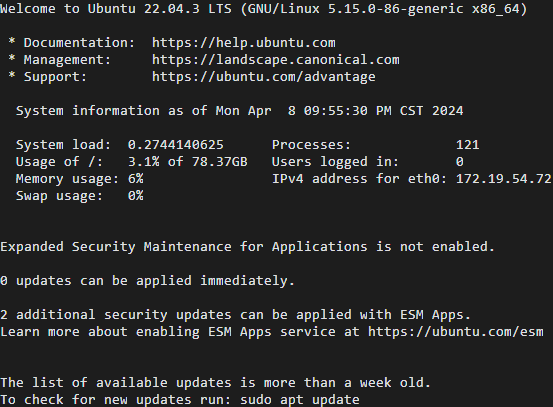
\includegraphics[width=0.8\textwidth]{figures/ServerVersion.png}
    \caption{服务器版本信息}
    \label{fig:ServerVersion}
\end{figure}

\begin{longtable}[c]{@{}lrll@{}}
    \caption{防火墙规则}
    \label{tab:FirewallRules}                                                 \\
    \toprule
    \textbf{协议} & \textbf{端口范围} & \textbf{限制IP来源} & \textbf{备注}               \\ \midrule
    \endfirsthead
    \multicolumn{4}{r}{\textbf{续表~\thetable}}                                 \\
    \toprule
    \textbf{协议} & \textbf{端口范围} & \textbf{限制IP来源} & \textbf{备注}               \\ \midrule
    \endhead
    \hline
    \multicolumn{4}{r}{续下页}
    \endfoot
    \endlastfoot
    TCP         & 80            & 0.0.0.0/0       & HTTP 默认端口                 \\
    TCP         & 443           & 0.0.0.0/0       & HTTPS 默认端口                \\
    TCP         & 1521          & 0.0.0.0/0       & PetJoy Oracle Database 端口 \\
    TCP         & 5101          & 0.0.0.0/0       & PetJoy DatabaseWebAPI 端口  \\
    TCP         & 22            & 0.0.0.0/0       & SSH 远程服务默认端口              \\ \bottomrule
\end{longtable}

\paragraph{部署Docker环境}

部署Docker环境的流程如下:

\begin{enumerate}
    \item 设置Docker的apt仓库
          \begin{minted}[baselinestretch=1]{bash}
# Add Docker's official GPG key:
sudo apt-get update
sudo apt-get install ca-certificates curl
sudo install -m 0755 -d /etc/apt/keyrings
sudo curl -fsSL https://download.docker.com/linux/ubuntu/gpg -o /etc/apt/keyrings/docker.asc
sudo chmod a+r /etc/apt/keyrings/docker.asc

# Add the repository to Apt sources:
echo \
  "deb [arch=$(dpkg --print-architecture) signed-by=/etc/apt/keyrings/docker.asc] https://download.docker.com/linux/ubuntu \
  $(. /etc/os-release && echo "$VERSION_CODENAME") stable" | \
  sudo tee /etc/apt/sources.list.d/docker.list > /dev/null
sudo apt-get update
          \end{minted}
    \item 安装Docker
          \begin{minted}[baselinestretch=1]{bash}
sudo apt-get install docker-ce docker-ce-cli containerd.io docker-buildx-plugin docker-compose-plugin
          \end{minted}
    \item 查看Docker版本,验证Docker安装是否成功(\cref{fig:ClientDockerVersion}、\cref{fig:ServerDockerVersion})
          \begin{minted}[baselinestretch=1]{bash}
docker version
          \end{minted}
\end{enumerate}

\begin{figure}[htbp]
    \centering
    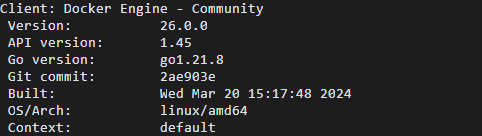
\includegraphics[width=0.8\textwidth]{figures/ClientDockerVersion.png}
    \caption{客户端Docker版本信息}
    \label{fig:ClientDockerVersion}
\end{figure}

\begin{figure}[htbp]
    \centering
    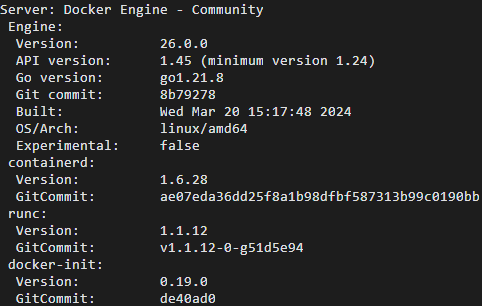
\includegraphics[width=0.8\textwidth]{figures/ServerDockerVersion.png}
    \caption{服务端Docker版本信息}
    \label{fig:ServerDockerVersion}
\end{figure}

\paragraph{数据持久化方式部署Oracle 12c数据库}

数据持久化方式部署Oracle 12c数据库的流程如下:

\begin{enumerate}
    \item 下载镜像文件
          \begin{minted}[baselinestretch=1]{bash}
docker pull absolutapps/oracle-12c-ee:latest
          \end{minted}
    \item 查看镜像文件
          \begin{minted}[baselinestretch=1]{bash}
docker images
          \end{minted}
    \item 创建主机内路径
          \begin{minted}[baselinestretch=1]{bash}
mkdir -p /home/local/oracle-data
          \end{minted}
    \item 在 Docker 容器内运行 Oracle 12c 数据库
          \begin{minted}[baselinestretch=1]{bash}
docker run -d --name petjoy-oracle-database --privileged -v /home/local/oracle-data:/u01/app/oracle -p 8080:8080 -p 1521:1521 absolutapps/oracle-12c-ee
          \end{minted}
    \item 查看容器启动日志(\cref{fig:ContainerStartupLog})
          \begin{minted}[baselinestretch=1]{bash}
docker logs -f petjoy-oracle-database
          \end{minted}
    \item 查看容器状态
          \begin{minted}[baselinestretch=1]{bash}
docker ps
          \end{minted}
\end{enumerate}

\begin{figure}[htbp]
    \centering
    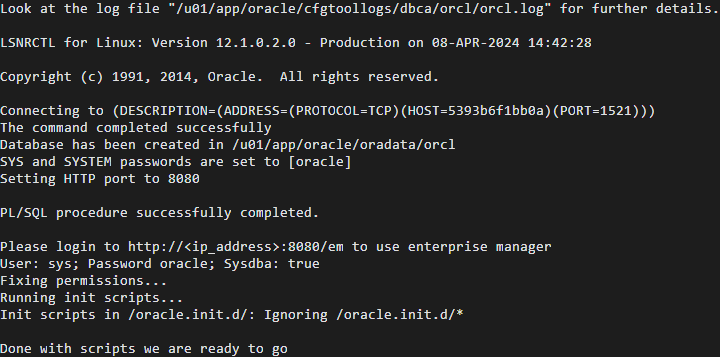
\includegraphics[width=0.8\textwidth]{figures/ContainerStartupLog.png}
    \caption{容器启动日志}
    \label{fig:ContainerStartupLog}
\end{figure}

\paragraph{测试Oracle 12c数据库}

测试Oracle 12c数据库的流程如下:

\begin{enumerate}
    \item 进入容器
          \begin{minted}[baselinestretch=1]{bash}
docker exec -it petjoy-oracle-database /bin/bash
          \end{minted}
    \item 切换数据库用户
          \begin{minted}[baselinestretch=1]{bash}
su oracle
          \end{minted}
    \item 进入数据库(\cref{fig:AccessToDatabase})
          \begin{minted}[baselinestretch=1]{bash}
$ORACLE_HOME/bin/sqlplus / as sysdba
          \end{minted}
    \item 查询数据库状态
          \begin{minted}[baselinestretch=1]{sql}
select status from v$instance;
          \end{minted}
\end{enumerate}

\begin{figure}[htbp]
    \centering
    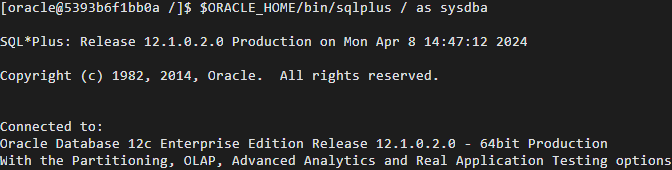
\includegraphics[width=0.8\textwidth]{figures/AccessToDatabase.png}
    \caption{进入数据库}
    \label{fig:AccessToDatabase}
\end{figure}

\paragraph{添加Oracle 12c数据库用户}

添加Oracle 12c数据库用户的流程如下:

\begin{enumerate}
    \item 连接到数据库作为 SYSDBA
          \begin{minted}[baselinestretch=1]{sql}
conn system/oracle as sysdba;
          \end{minted}
    \item 修改 system 用户的密码为 oracle
          \begin{minted}[baselinestretch=1]{sql}
alter user system identified by oracle;
          \end{minted}
    \item 修改 sys 用户的密码为 sys
          \begin{minted}[baselinestretch=1]{sql}
alter user sys identified by sys;
          \end{minted}
    \item 修改默认的密码策略,将密码的有效期限设置为无限
          \begin{minted}[baselinestretch=1]{sql}
ALTER PROFILE DEFAULT LIMIT PASSWORD_LIFE_TIME UNLIMITED;
          \end{minted}
    \item 创建一个新用户 tjsse\_dbteam,并且设置其密码为 tjsse2024
          \begin{minted}[baselinestretch=1]{sql}
create user tjsse_dbteam identified by tjsse2024;
          \end{minted}
    \item 为 tjsse\_dbteam 用户授权
          \begin{minted}[baselinestretch=1]{sql}
grant connect, resource, dba to tjsse_dbteam;
          \end{minted}
    \item 查询数据库账户
          \begin{minted}[baselinestretch=1]{sql}
SELECT username FROM dba_users;
          \end{minted}
\end{enumerate}

\paragraph{以tjsse\_dbteam用户身份连接数据库}

可以通过轻量应用服务器和JetBrains DataGrip以tjsse\_dbteam用户身份连接数据库。

\subparagraph{通过轻量应用服务器连接数据库}

通过轻量应用服务器连接数据库的流程如下:

\begin{enumerate}
    \item 进入容器
          \begin{minted}[baselinestretch=1]{bash}
docker exec -it petjoy-oracle-database /bin/bash
          \end{minted}
    \item 切换数据库用户
          \begin{minted}[baselinestretch=1]{bash}
su oracle
          \end{minted}
    \item 进入数据库
          \begin{minted}[baselinestretch=1]{bash}
$ORACLE_HOME/bin/sqlplus
          \end{minted}
    \item 输入用户名和密码
\end{enumerate}

\subparagraph{通过JetBrains DataGrip连接数据库}

通过JetBrains DataGrip连接数据库(\cref{fig:ConnectViaDataGrip}):

\begin{figure}[htbp]
    \centering
    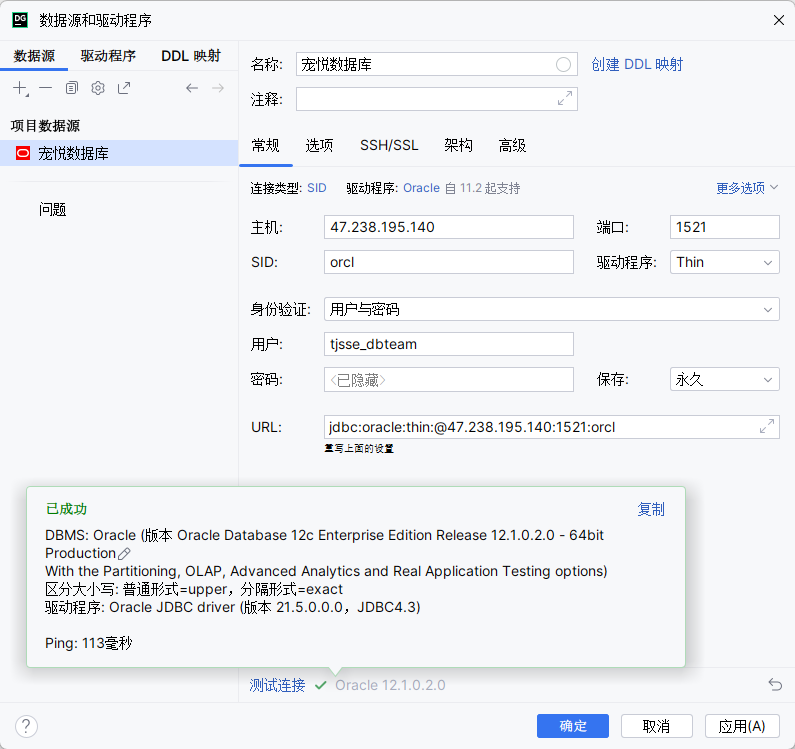
\includegraphics[width=\textwidth]{figures/ConnectViaDataGrip.png}
    \caption{通过JetBrains DataGrip连接数据库}
    \label{fig:ConnectViaDataGrip}
\end{figure}

\begin{itemize}
    \item \textbf{主机}:47.238.195.140
    \item \textbf{端口}:1521
    \item \textbf{SID}:orcl
    \item \textbf{驱动程序}:Thin
    \item \textbf{身份验证}:用户与密码
    \item \textbf{用户}:tjsse\_dbteam
    \item \textbf{密码}:tjsse2024
    \item \textbf{保存}:永久
    \item \textbf{URL}:jdbc:oracle:thin:@47.238.195.140:1521:orcl
\end{itemize}

\subsubsection{扩展性和可维护性}

在数据库设计中,扩展性和可维护性是确保数据库系统能够适应不断变化的业务需求和数据增长的重要因素。良好的设计可以使数据库在处理更大的数据量、更高的并发请求以及不断变化的业务需求时,仍然保持高效、稳定的运行。

本数据库使用了模块化设计。模块化设计是指将数据库结构划分为多个独立的模块,每个模块负责特定的功能或业务。这种设计有助于简化数据库管理和维护。通过将不同业务模块分开设计,以便独立开发和维护。

\subsection{数据定义语言(DDL)设计}

对于数据库设计,确保有效的数据定义语言(DDL)实现是至关重要的。基于数据库设计的规范化、主键和索引、外键、数据类型和约束、安全性和隐私、性能优化、数据持久化、扩展性和可维护性等方面,我们对各种表进行了数据定义语言(DDL)的设计。

\subsubsection{用户表 USER}

下面是用户表 USER 的数据定义语言:

\begin{minted}[baselinestretch=1]{sql}
create table "USER"
(
    user_id             INT           GENERATED ALWAYS AS IDENTITY (START WITH 1 INCREMENT BY 1) not null
        constraint USER_pk
            primary key,
    user_name           VARCHAR(64)   not null
        constraint user_name_uk
            unique,
    password            VARCHAR(64)   not null,
    email               VARCHAR(2048)
        constraint email_uk
            unique,
    registration_date   DATE          not null,
    last_login_time     DATE          not null,
    role                NUMBER(1)     not null,
    status              NUMBER(1)     not null,
    avatar_url          VARCHAR(2048),
    profile             VARCHAR(512),
    gender              NUMBER(1)     not null,
    birthdate           DATE          not null,
    experience_points   INT           not null,
    follows_count       INT           not null,
    followed_count      INT           not null,
    favorites_count     INT           not null,
    favorited_count     INT           not null,
    likes_count         INT           not null,
    liked_count         INT           not null,
    message_count       INT           not null
);

comment on table "USER" is '用户';
comment on column "USER".user_id is '用户ID';
comment on column "USER".user_name is '用户名';
comment on column "USER".password is '密码';
comment on column "USER".telephone is '手机号码';
comment on column "USER".registration_date is '注册日期';
comment on column "USER".last_login_time is '上次登录时间';
comment on column "USER".role is '用户角色';
comment on column "USER".status is '用户状态';
comment on column "USER".avatar_url is '头像链接';
comment on column "USER".profile is '个人简介';
comment on column "USER".gender is '性别';
comment on column "USER".birthdate is '出生日期';
comment on column "USER".experience_points is '经验点数';
comment on column "USER".follows_count is '关注数';
comment on column "USER".followed_count is '被关注数';
comment on column "USER".favorites_count is '收藏数';
comment on column "USER".favorited_count is '被收藏数';
comment on column "USER".likes_count is '点赞数';
comment on column "USER".liked_count is '被点赞数';
comment on column "USER".message_count is '留言数';
\end{minted}

\subsubsection{用户设置表 USER\_SETTING}

下面是用户设置表 USER\_SETTING 的数据定义语言:

\begin{minted}[baselinestretch=1]{sql}
create table USER_SETTING
(
    user_id                     INT       not null
        constraint USER_SETTING_pk
            primary key
        constraint USER_SETTING_USER_fk
            references "USER" ON DELETE CASCADE,
    is_telephone_public         NUMBER(1) not null,
    is_registration_date_public NUMBER(1) not null,
    is_profile_public           NUMBER(1) not null,
    is_gender_public            NUMBER(1) not null,
    is_birthdate_public         NUMBER(1) not null,
    is_level_public             NUMBER(1) not null,
    is_following_count_public   NUMBER(1) not null,
    is_followers_count_public   NUMBER(1) not null,
    is_favorites_count_public   NUMBER(1) not null,
    is_favored_count_public     NUMBER(1) not null,
    is_likes_count_public       NUMBER(1) not null,
    is_liked_count_public       NUMBER(1) not null,
    is_message_count_public     NUMBER(1) not null,
    allow_following             NUMBER(1) not null,
    receive_admin_notifications NUMBER(1) not null,
    receive_user_notifications  NUMBER(1) not null
);

comment on table USER_SETTING is '用户设置';
comment on column USER_SETTING.user_id is '用户ID';
comment on column USER_SETTING.is_telephone_public is '是否公开手机号码';
comment on column USER_SETTING.is_registration_date_public is '是否公开注册日期';
comment on column USER_SETTING.is_profile_public is '是否公开个人简介';
comment on column USER_SETTING.is_gender_public is '是否公开性别';
comment on column USER_SETTING.is_birthdate_public is '是否公开出生日期';
comment on column USER_SETTING.is_level_public is '是否公开等级';
comment on column USER_SETTING.is_following_count_public is '是否公开关注数';
comment on column USER_SETTING.is_followers_count_public is '是否公开被关注数';
comment on column USER_SETTING.is_favorites_count_public is '是否公开收藏数';
comment on column USER_SETTING.is_favored_count_public is '是否公开被收藏数';
comment on column USER_SETTING.is_likes_count_public is '是否公开点赞数';
comment on column USER_SETTING.is_liked_count_public is '是否公开被点赞数';
comment on column USER_SETTING.is_message_count_public is '是否公开留言数';
comment on column USER_SETTING.allow_following is '是否允许他人关注';
comment on column USER_SETTING.receive_admin_notifications is '是否接受管理员通知';
comment on column USER_SETTING.receive_user_notifications is '是否接受用户通知';
\end{minted}

\subsubsection{用户打卡表 USER\_CHECK\_IN}

下面是用户打卡表 USER\_CHECK\_IN 的数据定义语言:

\begin{minted}[baselinestretch=1]{sql}
create table USER_CHECK_IN
(
    check_in_id   INT  GENERATED ALWAYS AS IDENTITY (START WITH 1 INCREMENT BY 1) not null
        constraint USER_CHECK_IN_pk
            primary key,
    user_id       INT  not null
        constraint USER_CHECK_IN_USER_fk
            references "USER" ON DELETE CASCADE,
    check_in_time DATE not null
);

comment on table USER_CHECK_IN is '用户打卡';
comment on column USER_CHECK_IN.check_in_id is '打卡记录ID';
comment on column USER_CHECK_IN.user_id is '用户ID';
comment on column USER_CHECK_IN.check_in_time is '打卡时间';
\end{minted}

\subsubsection{用户关注表 USER\_FOLLOW}

下面是用户关注表 USER\_FOLLOW 的数据定义语言:

\begin{minted}[baselinestretch=1]{sql}
create table USER_FOLLOW
(
    user_id     INT  not null
        constraint USER_FOLLOW_USER_fk_1
            references "USER" ON DELETE CASCADE,
    follower_id INT  not null
        constraint USER_FOLLOW_USER_fk_2
            references "USER" ON DELETE CASCADE,
    follow_time DATE not null,
    constraint USER_FOLLOW_pk
        primary key (user_id, follower_id)
);

comment on table USER_FOLLOW is '用户关注';
comment on column USER_FOLLOW.user_id is '被关注者ID';
comment on column USER_FOLLOW.follower_id is '关注者ID';
comment on column USER_FOLLOW.follow_time is '关注时间';
\end{minted}

\subsubsection{用户留言表 USER\_MESSAGE}

下面是用户留言表 USER\_MESSAGE 的数据定义语言:

\begin{minted}[baselinestretch=1]{sql}
create table USER_MESSAGE
(
    message_id   INT          GENERATED ALWAYS AS IDENTITY (START WITH 1 INCREMENT BY 1) not null
        constraint USER_MESSAGE_pk
            primary key,
    user_id      INT          not null
        constraint USER_MESSAGE_USER_fk_1
            references "USER" ON DELETE CASCADE,
    commenter_id INT          not null
        constraint USER_MESSAGE_USER_fk_2
            references "USER" ON DELETE CASCADE,
    message      VARCHAR(512) not null,
    comment_time DATE         not null
);

comment on table USER_MESSAGE is '用户留言';
comment on column USER_MESSAGE.message_id is '留言ID';
comment on column USER_MESSAGE.user_id is '用户ID';
comment on column USER_MESSAGE.commenter_id is '留言者ID';
comment on column USER_MESSAGE.message is '留言内容';
comment on column USER_MESSAGE.comment_time is '留言时间';
\end{minted}

\subsubsection{用户反馈表 USER\_FEEDBACK}

下面是用户反馈表 USER\_FEEDBACK 的数据定义语言:

\begin{minted}[baselinestretch=1]{sql}
create table USER_FEEDBACK
(
    feedback_id       INTEGER       GENERATED ALWAYS AS IDENTITY (START WITH 1 INCREMENT BY 1) not null
        constraint USER_FEEDBACK_pk
            primary key,
    feedback_category VARCHAR(32)   not null,
    feedback_content  VARCHAR(2048) not null,
    feedback_time     DATE          not null,
    email             VARCHAR(2048),
    telephone         VARCHAR(16)
);

comment on table USER_FEEDBACK is '用户反馈';
comment on column USER_FEEDBACK.feedback_id is '反馈意见ID';
comment on column USER_FEEDBACK.feedback_category is '反馈类型';
comment on column USER_FEEDBACK.feedback_content is '反馈内容';
comment on column USER_FEEDBACK.feedback_time is '反馈时间';
comment on column USER_FEEDBACK.email is '电子邮箱';
comment on column USER_FEEDBACK.telephone is '手机号码';
\end{minted}

\subsubsection{帖子分类表 POST\_CATEGORY}

下面是帖子分类表 POST\_CATEGORY 的数据定义语言:

\begin{minted}[baselinestretch=1]{sql}
create table POST_CATEGORY
(
    category_id INT         not null
        constraint POST_CATEGORY_pk
            primary key,
    category    VARCHAR(64) not null
        constraint post_category_uk
            unique
);

comment on table POST_CATEGORY is '帖子分类';
comment on column POST_CATEGORY.category_id is '帖子分类ID';
comment on column POST_CATEGORY.category is '帖子分类';
\end{minted}

\subsubsection{帖子表 POST}

下面是帖子表 POST 的数据定义语言:

\begin{minted}[baselinestretch=1]{sql}
create table POST
(
    post_id        INT           GENERATED ALWAYS AS IDENTITY (START WITH 1 INCREMENT BY 1) not null
        constraint POST_pk
            primary key,
    user_id        INT           not null
        constraint POST_USER_fk
            references "USER" ON DELETE CASCADE,
    category_id    INT           not null
        constraint POST_POST_CATEGORY_fk
            references POST_CATEGORY (category_id) ON DELETE CASCADE,
    title          VARCHAR(256)  not null,
    content        VARCHAR(2048) not null,
    creation_date  DATE          not null,
    update_date    DATE          not null,
    is_sticky      NUMBER(1)     not null,
    like_count     INT           not null,
    dislike_count  INT           not null,
    favorite_count INT           not null,
    comment_count  INT           not null,
    image_url      VARCHAR(2048)
);

comment on table POST is '帖子';
comment on column POST.post_id is '帖子ID';
comment on column POST.user_id is '发帖用户ID';
comment on column POST.category_id is '帖子分类ID';
comment on column POST.title is '标题';
comment on column POST.content is '内容';
comment on column POST.creation_date is '创建时间';
comment on column POST.update_date is '更新时间';
comment on column POST.is_sticky is '是否置顶';
comment on column POST.like_count is '点赞数';
comment on column POST.dislike_count is '点踩数';
comment on column POST.favorite_count is '收藏数';
comment on column POST.comment_count is '评论数';
comment on column POST.image_url is '图片链接';
\end{minted}

\subsubsection{帖子评论表 POST\_COMMENT}

下面是帖子评论表 POST\_COMMENT 的数据定义语言:

\begin{minted}[baselinestretch=1]{sql}
create table POST_COMMENT
(
    comment_id        INT          GENERATED ALWAYS AS IDENTITY (START WITH 1 INCREMENT BY 1) not null
        constraint POST_COMMENT_pk
            primary key,
    post_id           INT          not null
        constraint POST_COMMENT_POST_fk
            references POST ON DELETE CASCADE,
    user_id           INT          not null
        constraint POST_COMMENT_USER_fk
            references "USER" ON DELETE CASCADE,
    parent_comment_id INT
        constraint POST_COMMENT_POST_COMMENT_fk
            references POST_COMMENT ON DELETE CASCADE,
    content           VARCHAR(512) not null,
    comment_time      DATE         not null,
    like_count        INT          not null,
    dislike_count     INT          not null
);

comment on table POST_COMMENT is '帖子评论';
comment on column POST_COMMENT.comment_id is '帖子评论ID';
comment on column POST_COMMENT.post_id is '帖子ID';
comment on column POST_COMMENT.user_id is '用户ID';
comment on column POST_COMMENT.parent_comment_id is '父评论ID';
comment on column POST_COMMENT.content is '评论内容';
comment on column POST_COMMENT.comment_time is '评论时间';
comment on column POST_COMMENT.like_count is '点赞数';
comment on column POST_COMMENT.dislike_count is '点踩数';
\end{minted}

\subsubsection{帖子点赞表 POST\_LIKE}

下面是帖子点赞表 POST\_LIKE 的数据定义语言:

\begin{minted}[baselinestretch=1]{sql}
create table POST_LIKE
(
    post_id   INT  not null
        constraint POST_LIKE_POST_fk
            references POST ON DELETE CASCADE,
    user_id   INT  not null
        constraint POST_LIKE_USER_fk
            references "USER" ON DELETE CASCADE,
    like_time DATE not null,
    constraint POST_LIKE_pk
        primary key (post_id, user_id)
);

comment on table POST_LIKE is '帖子点赞';
comment on column POST_LIKE.post_id is '帖子ID';
comment on column POST_LIKE.user_id is '用户ID';
comment on column POST_LIKE.like_time is '点赞时间';
\end{minted}

\subsubsection{帖子点踩表 POST\_DISLIKE}

下面是帖子点踩表 POST\_DISLIKE 的数据定义语言:

\begin{minted}[baselinestretch=1]{sql}
create table POST_DISLIKE
(
    post_id      INT  not null
        constraint POST_DISLIKE_POST_fk
            references POST ON DELETE CASCADE,
    user_id      INT  not null
        constraint POST_DISLIKE_USER_fk
            references "USER" ON DELETE CASCADE,
    dislike_time DATE not null,
    constraint POST_DISLIKE_pk
        primary key (post_id, user_id)
);

comment on table POST_DISLIKE is '帖子点踩';
comment on column POST_DISLIKE.post_id is '帖子ID';
comment on column POST_DISLIKE.user_id is '用户ID';
comment on column POST_DISLIKE.dislike_time is '点踩时间';
\end{minted}

\subsubsection{帖子评论点赞表 POST\_COMMENT\_LIKE}

下面是帖子评论点赞表 POST\_COMMENT\_LIKE 的数据定义语言:

\begin{minted}[baselinestretch=1]{sql}
create table POST_COMMENT_LIKE
(
    comment_id INT  not null
        constraint POST_COMMENT_LPC_fk
            references POST_COMMENT ON DELETE CASCADE,
    user_id    INT  not null
        constraint POST_COMMENT_LIKE_USER_fk
            references "USER" ON DELETE CASCADE,
    like_time  DATE not null,
    constraint POST_COMMENT_LIKE_pk
        primary key (comment_id, user_id)
);

comment on table POST_COMMENT_LIKE is '帖子评论点赞';
comment on column POST_COMMENT_LIKE.comment_id is '帖子评论ID';
comment on column POST_COMMENT_LIKE.user_id is '用户ID';
comment on column POST_COMMENT_LIKE.like_time is '点赞时间';
\end{minted}

\subsubsection{帖子评论点踩表 POST\_COMMENT\_DISLIKE}

下面是帖子评论点踩表 POST\_COMMENT\_DISLIKE 的数据定义语言:

\begin{minted}[baselinestretch=1]{sql}
create table POST_COMMENT_DISLIKE
(
    comment_id   INT  not null
        constraint POST_COMMENT_DPC_fk
            references POST_COMMENT ON DELETE CASCADE,
    user_id      INT  not null
        constraint POST_COMMENT_DISLIKE_USER_fk
            references "USER" ON DELETE CASCADE,
    dislike_time DATE not null,
    constraint POST_COMMENT_DISLIKE_pk
        primary key (comment_id, user_id)
);

comment on table POST_COMMENT_DISLIKE is '帖子评论点踩';
comment on column POST_COMMENT_DISLIKE.comment_id is '帖子评论ID';
comment on column POST_COMMENT_DISLIKE.user_id is '用户ID';
comment on column POST_COMMENT_DISLIKE.dislike_time is '点踩时间';
\end{minted}

\subsubsection{帖子收藏表 POST\_FAVORITE}

下面是帖子收藏表 POST\_FAVORITE 的数据定义语言:

\begin{minted}[baselinestretch=1]{sql}
create table POST_FAVORITE
(
    post_id       INT  not null
        constraint POST_FAVORITE_POST_fk
            references POST ON DELETE CASCADE,
    user_id       INT  not null
        constraint POST_FAVORITE_USER_fk
            references "USER" ON DELETE CASCADE,
    favorite_time DATE not null,
    constraint POST_FAVORITE_pk
        primary key (post_id, user_id)
);

comment on table POST_FAVORITE is '帖子收藏';
comment on column POST_FAVORITE.post_id is '帖子ID';
comment on column POST_FAVORITE.user_id is '用户ID';
comment on column POST_FAVORITE.favorite_time is '收藏时间';
\end{minted}

\subsubsection{帖子举报表 POST\_REPORT}

下面是帖子举报表 POST\_REPORT 的数据定义语言:

\begin{minted}[baselinestretch=1]{sql}
create table POST_REPORT
(
    post_report_id   INT          GENERATED ALWAYS AS IDENTITY (START WITH 1 INCREMENT BY 1) not null
        constraint POST_REPORT_pk
            primary key,
    reporter_id      INT          not null
        constraint POST_REPORT_USER_fk_1
            references "USER" ON DELETE CASCADE,
    reported_user_id INT          not null
        constraint POST_REPORT_USER_fk_2
            references "USER" ON DELETE CASCADE,
    reported_post_id INT          not null
        constraint POST_REPORT_POST_fk
            references POST ON DELETE CASCADE,
    report_reason    VARCHAR(512) not null,
    report_time      DATE         not null,
    status           NUMBER(1)    not null
);

comment on table POST_REPORT is '帖子举报';
comment on column POST_REPORT.post_report_id is '帖子举报ID';
comment on column POST_REPORT.reporter_id is '举报者ID';
comment on column POST_REPORT.reported_user_id is '被举报者ID';
comment on column POST_REPORT.reported_post_id is '被举报帖子ID';
comment on column POST_REPORT.report_reason is '举报原因';
comment on column POST_REPORT.report_time is '举报时间';
comment on column POST_REPORT.status is '处理状态';
\end{minted}

\subsubsection{帖子评论举报表 POST\_COMMENT\_REPORT}

下面是帖子评论举报表 POST\_COMMENT\_REPORT 的数据定义语言:

\begin{minted}[baselinestretch=1]{sql}
create table POST_COMMENT_REPORT
(
    post_comment_report_id INT          GENERATED ALWAYS AS IDENTITY (START WITH 1 INCREMENT BY 1) not null
        constraint POST_COMMENT_REPORT_pk
            primary key,
    reporter_id            INT          not null
        constraint POST_COMMENT_REPORT_USER_fk_1
            references "USER" ON DELETE CASCADE,
    reported_user_id       INT          not null
        constraint POST_COMMENT_REPORT_USER_fk_2
            references "USER" ON DELETE CASCADE,
    reported_post_id       INT          not null
        constraint POST_COMMENT_REPORT_POST_fk
            references POST ON DELETE CASCADE,
    reported_comment_id    INT          not null
        constraint POST_COMMENT_REPORT_PC_fk
            references POST_COMMENT ON DELETE CASCADE,
    report_reason          VARCHAR(512) not null,
    report_time            DATE         not null,
    status                 NUMBER(1)    not null
);

comment on table POST_COMMENT_REPORT is '帖子评论举报';
comment on column POST_COMMENT_REPORT.post_comment_report_id is '帖子评论举报ID';
comment on column POST_COMMENT_REPORT.reporter_id is '举报者ID';
comment on column POST_COMMENT_REPORT.reported_user_id is '被举报者ID';
comment on column POST_COMMENT_REPORT.reported_post_id is '被举报评论所属帖子ID';
comment on column POST_COMMENT_REPORT.reported_comment_id is '被举报评论ID';
comment on column POST_COMMENT_REPORT.report_reason is '举报原因';
comment on column POST_COMMENT_REPORT.report_time is '举报时间';
comment on column POST_COMMENT_REPORT.status is '处理状态';
\end{minted}

\subsubsection{新闻标签表 NEWS\_TAG}

下面是新闻标签表 NEWS\_TAG 的数据定义语言:

\begin{minted}[baselinestretch=1]{sql}
create table NEWS_TAG
(
    tag_id INT         not null
        constraint NEWS_TAG_pk
            primary key,
    tag    VARCHAR(64) not null
        constraint tag_uk
            unique
);

comment on table NEWS_TAG is '新闻标签';
comment on column NEWS_TAG.tag_id is '新闻标签ID';
comment on column NEWS_TAG.tag is '新闻标签';
\end{minted}

\subsubsection{新闻表 NEWS}

下面是新闻表 NEWS 的数据定义语言:

\begin{minted}[baselinestretch=1]{sql}
create table NEWS
(
    news_id        INT           GENERATED ALWAYS AS IDENTITY (START WITH 1 INCREMENT BY 1) not null
        constraint NEWS_pk
            primary key,
    user_id        INT           not null
        constraint NEWS_USER_fk
            references "USER" ON DELETE CASCADE,
    tag_id         INT           not null
        constraint NEWS_NEWS_TAG_fk
            references NEWS_TAG (tag_id) ON DELETE CASCADE,
    title          VARCHAR(256)  not null,
    summary        VARCHAR(512)  not null,
    content        CLOB          not null,
    creation_date  DATE          not null,
    update_date    DATE          not null,
    cover_url      VARCHAR(2048) not null,
    is_sticky      NUMBER(1)     not null,
    like_count     INT           not null,
    dislike_count  INT           not null,
    favorite_count INT           not null,
    comment_count  INT           not null
);

comment on table NEWS is '新闻';
comment on column NEWS.news_id is '新闻ID';
comment on column NEWS.user_id is '管理员ID';
comment on column NEWS.tag_id is '新闻标签ID';
comment on column NEWS.title is '标题';
comment on column NEWS.summary is '新闻摘要';
comment on column NEWS.content is '内容';
comment on column NEWS.creation_date is '创建时间';
comment on column NEWS.update_date is '更新时间';
comment on column NEWS.cover_url is '封面图片链接';
comment on column NEWS.is_sticky is '是否置顶';
comment on column NEWS.like_count is '点赞数';
comment on column NEWS.dislike_count is '点踩数';
comment on column NEWS.favorite_count is '收藏数';
comment on column NEWS.comment_count is '评论数';
\end{minted}

\subsubsection{新闻评论表 NEWS\_COMMENT}

下面是新闻评论表 NEWS\_COMMENT 的数据定义语言:

\begin{minted}[baselinestretch=1]{sql}
create table NEWS_COMMENT
(
    comment_id        INT          GENERATED ALWAYS AS IDENTITY (START WITH 1 INCREMENT BY 1) not null
        constraint NEWS_COMMENT_pk
            primary key,
    news_id           INT          not null
        constraint NEWS_COMMENT_NEWS_fk
            references NEWS ON DELETE CASCADE,
    user_id           INT          not null
        constraint NEWS_COMMENT_USER_fk
            references "USER" ON DELETE CASCADE,
    parent_comment_id INT
        constraint NEWS_COMMENT_NEWS_COMMENT_fk
            references NEWS_COMMENT ON DELETE CASCADE,
    content           VARCHAR(512) not null,
    comment_time      DATE         not null,
    like_count        INT          not null,
    dislike_count     INT          not null
);

comment on table NEWS_COMMENT is '新闻评论';
comment on column NEWS_COMMENT.comment_id is '新闻评论ID';
comment on column NEWS_COMMENT.news_id is '新闻ID';
comment on column NEWS_COMMENT.user_id is '用户ID';
comment on column NEWS_COMMENT.parent_comment_id is '父评论ID';
comment on column NEWS_COMMENT.content is '评论内容';
comment on column NEWS_COMMENT.comment_time is '评论时间';
comment on column NEWS_COMMENT.like_count is '点赞数';
comment on column NEWS_COMMENT.dislike_count is '点踩数';
\end{minted}

\subsubsection{新闻点赞表 NEWS\_LIKE}

下面是新闻点赞表 NEWS\_LIKE 的数据定义语言:

\begin{minted}[baselinestretch=1]{sql}
create table NEWS_LIKE
(
    news_id   INT  not null
        constraint NEWS_LIKE_NEWS_fk
            references NEWS ON DELETE CASCADE,
    user_id   INT  not null
        constraint NEWS_LIKE_USER_fk
            references "USER" ON DELETE CASCADE,
    like_time DATE not null,
    constraint NEWS_LIKE_pk
        primary key (news_id, user_id)
);

comment on table NEWS_LIKE is '新闻点赞';
comment on column NEWS_LIKE.news_id is '新闻ID';
comment on column NEWS_LIKE.user_id is '用户ID';
comment on column NEWS_LIKE.like_time is '点赞时间';
\end{minted}

\subsubsection{新闻点踩表 NEWS\_DISLIKE}

下面是新闻点踩表 NEWS\_DISLIKE 的数据定义语言:

\begin{minted}[baselinestretch=1]{sql}
create table NEWS_DISLIKE
(
    news_id      INT  not null
        constraint NEWS_DISLIKE_NEWS_fk
            references NEWS ON DELETE CASCADE,
    user_id      INT  not null
        constraint NEWS_DISLIKE_USER_fk
            references "USER" ON DELETE CASCADE,
    dislike_time DATE not null,
    constraint NEWS_DISLIKE_pk
        primary key (news_id, user_id)
);

comment on table NEWS_DISLIKE is '新闻点踩';
comment on column NEWS_DISLIKE.news_id is '新闻ID';
comment on column NEWS_DISLIKE.user_id is '用户ID';
comment on column NEWS_DISLIKE.dislike_time is '点踩时间';
\end{minted}

\subsubsection{新闻评论点赞表 NEWS\_COMMENT\_LIKE}

下面是新闻评论点赞表 NEWS\_COMMENT\_LIKE 的数据定义语言:

\begin{minted}[baselinestretch=1]{sql}
create table NEWS_COMMENT_LIKE
(
    comment_id INT  not null
        constraint NEWS_COMMENT_LIKE_NC_fk
            references NEWS_COMMENT ON DELETE CASCADE,
    user_id    INT  not null
        constraint NEWS_COMMENT_LIKE_USER_fk
            references "USER" ON DELETE CASCADE,
    like_time  DATE not null,
    constraint NEWS_COMMENT_LIKE_pk
        primary key (comment_id, user_id)
);

comment on table NEWS_COMMENT_LIKE is '新闻评论点赞';
comment on column NEWS_COMMENT_LIKE.comment_id is '新闻评论ID';
comment on column NEWS_COMMENT_LIKE.user_id is '用户ID';
comment on column NEWS_COMMENT_LIKE.like_time is '点赞时间';
\end{minted}

\subsubsection{新闻评论点踩表 NEWS\_COMMENT\_DISLIKE}

下面是新闻评论点踩表 NEWS\_COMMENT\_DISLIKE 的数据定义语言:

\begin{minted}[baselinestretch=1]{sql}
create table NEWS_COMMENT_DISLIKE
(
    comment_id   INT  not null
        constraint NEWS_COMMENT_DISLIKE_NC_fk
            references NEWS_COMMENT ON DELETE CASCADE,
    user_id      INT  not null
        constraint NEWS_COMMENT_DISLIKE_USER_fk
            references "USER" ON DELETE CASCADE,
    dislike_time DATE not null,
    constraint NEWS_COMMENT_DISLIKE_pk
        primary key (comment_id, user_id)
);

comment on table NEWS_COMMENT_DISLIKE is '新闻评论点踩';
comment on column NEWS_COMMENT_DISLIKE.comment_id is '新闻评论ID';
comment on column NEWS_COMMENT_DISLIKE.user_id is '用户ID';
comment on column NEWS_COMMENT_DISLIKE.dislike_time is '点踩时间';
\end{minted}

\subsubsection{新闻收藏表 NEWS\_FAVORITE}

下面是新闻收藏表 NEWS\_FAVORITE 的数据定义语言:

\begin{minted}[baselinestretch=1]{sql}
create table NEWS_FAVORITE
(
    news_id       INT  not null
        constraint NEWS_FAVORITE_NEWS_fk
            references NEWS ON DELETE CASCADE,
    user_id       INT  not null
        constraint NEWS_FAVORITE_USER_fk
            references "USER" ON DELETE CASCADE,
    favorite_time DATE not null,
    constraint NEWS_FAVORITE_pk
        primary key (news_id, user_id)
);

comment on table NEWS_FAVORITE is '新闻收藏';
comment on column NEWS_FAVORITE.news_id is '新闻ID';
comment on column NEWS_FAVORITE.user_id is '用户ID';
comment on column NEWS_FAVORITE.favorite_time is '收藏时间';
\end{minted}

\subsubsection{新闻评论举报表 NEWS\_COMMENT\_REPORT}

下面是新闻评论举报表 NEWS\_COMMENT\_REPORT 的数据定义语言:

\begin{minted}[baselinestretch=1]{sql}
create table NEWS_COMMENT_REPORT
(
    news_comment_report_id INT          GENERATED ALWAYS AS IDENTITY (START WITH 1 INCREMENT BY 1) not null
        constraint NEWS_COMMENT_REPORT_pk
            primary key,
    reporter_id            INT          not null
        constraint NEWS_COMMENT_REPORT_USER_fk_1
            references "USER" ON DELETE CASCADE,
    reported_user_id       INT          not null
        constraint NEWS_COMMENT_REPORT_USER_fk_2
            references "USER" ON DELETE CASCADE,
    reported_news_id       INT          not null
        constraint NEWS_COMMENT_REPORT_NEWS_fk
            references NEWS ON DELETE CASCADE,
    reported_comment_id    INT          not null
        constraint NEWS_COMMENT_REPORT_NC_fk
            references NEWS_COMMENT ON DELETE CASCADE,
    report_reason          VARCHAR(512) not null,
    report_time            DATE         not null,
    status                 NUMBER(1)    not null
);

comment on table NEWS_COMMENT_REPORT is '新闻评论举报';
comment on column NEWS_COMMENT_REPORT.news_comment_report_id is '新闻评论举报ID';
comment on column NEWS_COMMENT_REPORT.reporter_id is '举报者ID';
comment on column NEWS_COMMENT_REPORT.reported_user_id is '被举报者ID';
comment on column NEWS_COMMENT_REPORT.reported_news_id is '被举报评论所属新闻ID';
comment on column NEWS_COMMENT_REPORT.reported_comment_id is '被举报评论ID';
comment on column NEWS_COMMENT_REPORT.report_reason is '举报原因';
comment on column NEWS_COMMENT_REPORT.report_time is '举报时间';
comment on column NEWS_COMMENT_REPORT.status is '处理状态';
\end{minted}

\subsubsection{宠物分类表 PET\_CATEGORY}

下面是宠物分类表 PET\_CATEGORY 的数据定义语言:

\begin{minted}[baselinestretch=1]{sql}
create table PET_CATEGORY
(
    category_id      INT           not null
        constraint PET_CATEGORY_pk
            primary key,
    category_name_zh VARCHAR(1024) not null
        constraint category_name_zh_uk
            unique,
    category_name_de VARCHAR(1024) not null
        constraint category_name_de_uk
            unique,
    category_name_en VARCHAR(1024) not null
        constraint category_name_en_uk
            unique,
    category_name_es VARCHAR(1024) not null
        constraint category_name_es_uk
            unique,
    category_name_fr VARCHAR(1024) not null
        constraint category_name_fr_uk
            unique,
    category_name_it VARCHAR(1024) not null
        constraint category_name_it_uk
            unique,
    category_name_ja VARCHAR(1024) not null
        constraint category_name_ja_uk
            unique,
    category_name_ko VARCHAR(1024) not null
        constraint category_name_ko_uk
            unique,
    category_name_pt VARCHAR(1024) not null
        constraint category_name_pt_uk
            unique,
    category_name_ru VARCHAR(1024) not null
        constraint category_name_ru_uk
            unique,
    description_zh   CLOB          not null,
    description_de   CLOB          not null,
    description_en   CLOB          not null,
    description_es   CLOB          not null,
    description_fr   CLOB          not null,
    description_it   CLOB          not null,
    description_ja   CLOB          not null,
    description_ko   CLOB          not null,
    description_pt   CLOB          not null,
    description_ru   CLOB          not null,
    image_url        VARCHAR(2048) not null
);

comment on table PET_CATEGORY is '宠物分类';
comment on column PET_CATEGORY.category_id is '宠物分类ID';
comment on column PET_CATEGORY.category_name_zh is '宠物分类名称(汉语)';
comment on column PET_CATEGORY.category_name_de is '宠物分类名称(德语)';
comment on column PET_CATEGORY.category_name_en is '宠物分类名称(英语)';
comment on column PET_CATEGORY.category_name_es is '宠物分类名称(西班牙语)';
comment on column PET_CATEGORY.category_name_fr is '宠物分类名称(法语)';
comment on column PET_CATEGORY.category_name_it is '宠物分类名称(意大利语)';
comment on column PET_CATEGORY.category_name_ja is '宠物分类名称(日语)';
comment on column PET_CATEGORY.category_name_ko is '宠物分类名称(韩语)';
comment on column PET_CATEGORY.category_name_pt is '宠物分类名称(葡萄牙语)';
comment on column PET_CATEGORY.category_name_ru is '宠物分类名称(俄语)';
comment on column PET_CATEGORY.description_zh is '描述(汉语)';
comment on column PET_CATEGORY.description_de is '描述(德语)';
comment on column PET_CATEGORY.description_en is '描述(英语)';
comment on column PET_CATEGORY.description_es is '描述(西班牙语)';
comment on column PET_CATEGORY.description_fr is '描述(法语)';
comment on column PET_CATEGORY.description_it is '描述(意大利语)';
comment on column PET_CATEGORY.description_ja is '描述(日语)';
comment on column PET_CATEGORY.description_ko is '描述(韩语)';
comment on column PET_CATEGORY.description_pt is '描述(葡萄牙语)';
comment on column PET_CATEGORY.description_ru is '描述(俄语)';
comment on column PET_CATEGORY.image_url is '图片链接';
\end{minted}

\subsubsection{宠物子类表 PET\_SUBCATEGORY}

下面是宠物子类表 PET\_SUBCATEGORY 的数据定义语言:

\begin{minted}[baselinestretch=1]{sql}
create table PET_SUBCATEGORY
(
    subcategory_id         INT           not null
        constraint PET_SUBCATEGORY_pk
            primary key,
    category_id            INT           not null
        constraint PET_SUBCATEGORY_PC_fk
            references PET_CATEGORY ON DELETE CASCADE,
    subcategory_name_zh    VARCHAR(1024) not null
        constraint subcategory_name_zh_uk
            unique,
    subcategory_name_de    VARCHAR(1024) not null
        constraint subcategory_name_de_uk
            unique,
    subcategory_name_en    VARCHAR(1024) not null
        constraint subcategory_name_en_uk
            unique,
    subcategory_name_es    VARCHAR(1024) not null
        constraint subcategory_name_es_uk
            unique,
    subcategory_name_fr    VARCHAR(1024) not null
        constraint subcategory_name_fr_uk
            unique,
    subcategory_name_it    VARCHAR(1024) not null
        constraint subcategory_name_it_uk
            unique,
    subcategory_name_ja    VARCHAR(1024) not null
        constraint subcategory_name_ja_uk
            unique,
    subcategory_name_ko    VARCHAR(1024) not null
        constraint subcategory_name_ko_uk
            unique,
    subcategory_name_pt    VARCHAR(1024) not null
        constraint subcategory_name_pt_uk
            unique,
    subcategory_name_ru    VARCHAR(1024) not null
        constraint subcategory_name_ru_uk
            unique,
    description_zh         CLOB          not null,
    description_de         CLOB          not null,
    description_en         CLOB          not null,
    description_es         CLOB          not null,
    description_fr         CLOB          not null,
    description_it         CLOB          not null,
    description_ja         CLOB          not null,
    description_ko         CLOB          not null,
    description_pt         CLOB          not null,
    description_ru         CLOB          not null,
    image_url              VARCHAR(2048) not null,
    origin_zh              VARCHAR(512)  not null,
    origin_de              VARCHAR(512)  not null,
    origin_en              VARCHAR(512)  not null,
    origin_es              VARCHAR(512)  not null,
    origin_fr              VARCHAR(512)  not null,
    origin_it              VARCHAR(512)  not null,
    origin_ja              VARCHAR(512)  not null,
    origin_ko              VARCHAR(512)  not null,
    origin_pt              VARCHAR(512)  not null,
    origin_ru              VARCHAR(512)  not null,
    size_zh                VARCHAR(512)  not null,
    size_de                VARCHAR(512)  not null,
    size_en                VARCHAR(512)  not null,
    size_es                VARCHAR(512)  not null,
    size_fr                VARCHAR(512)  not null,
    size_it                VARCHAR(512)  not null,
    size_ja                VARCHAR(512)  not null,
    size_ko                VARCHAR(512)  not null,
    size_pt                VARCHAR(512)  not null,
    size_ru                VARCHAR(512)  not null,
    coat_zh                VARCHAR(512)  not null,
    coat_de                VARCHAR(512)  not null,
    coat_en                VARCHAR(512)  not null,
    coat_es                VARCHAR(512)  not null,
    coat_fr                VARCHAR(512)  not null,
    coat_it                VARCHAR(512)  not null,
    coat_ja                VARCHAR(512)  not null,
    coat_ko                VARCHAR(512)  not null,
    coat_pt                VARCHAR(512)  not null,
    coat_ru                VARCHAR(512)  not null,
    lifespan_zh            VARCHAR(512)  not null,
    lifespan_de            VARCHAR(512)  not null,
    lifespan_en            VARCHAR(512)  not null,
    lifespan_es            VARCHAR(512)  not null,
    lifespan_fr            VARCHAR(512)  not null,
    lifespan_it            VARCHAR(512)  not null,
    lifespan_ja            VARCHAR(512)  not null,
    lifespan_ko            VARCHAR(512)  not null,
    lifespan_pt            VARCHAR(512)  not null,
    lifespan_ru            VARCHAR(512)  not null,
    temperament_zh         VARCHAR(512)  not null,
    temperament_de         VARCHAR(512)  not null,
    temperament_en         VARCHAR(512)  not null,
    temperament_es         VARCHAR(512)  not null,
    temperament_fr         VARCHAR(512)  not null,
    temperament_it         VARCHAR(512)  not null,
    temperament_ja         VARCHAR(512)  not null,
    temperament_ko         VARCHAR(512)  not null,
    temperament_pt         VARCHAR(512)  not null,
    temperament_ru         VARCHAR(512)  not null,
    diet_zh                VARCHAR(512)  not null,
    diet_de                VARCHAR(512)  not null,
    diet_en                VARCHAR(512)  not null,
    diet_es                VARCHAR(512)  not null,
    diet_fr                VARCHAR(512)  not null,
    diet_it                VARCHAR(512)  not null,
    diet_ja                VARCHAR(512)  not null,
    diet_ko                VARCHAR(512)  not null,
    diet_pt                VARCHAR(512)  not null,
    diet_ru                VARCHAR(512)  not null,
    latitude_and_longitude VARCHAR(512)  not null
);

comment on table PET_SUBCATEGORY is '宠物子类';
comment on column PET_SUBCATEGORY.subcategory_id is '宠物子类ID';
comment on column PET_SUBCATEGORY.category_id is '宠物分类ID';
comment on column PET_SUBCATEGORY.subcategory_name_zh is '宠物子类名称(汉语)';
comment on column PET_SUBCATEGORY.subcategory_name_de is '宠物子类名称(德语)';
comment on column PET_SUBCATEGORY.subcategory_name_en is '宠物子类名称(英语)';
comment on column PET_SUBCATEGORY.subcategory_name_es is '宠物子类名称(西班牙语)';
comment on column PET_SUBCATEGORY.subcategory_name_fr is '宠物子类名称(法语)';
comment on column PET_SUBCATEGORY.subcategory_name_it is '宠物子类名称(意大利语)';
comment on column PET_SUBCATEGORY.subcategory_name_ja is '宠物子类名称(日语)';
comment on column PET_SUBCATEGORY.subcategory_name_ko is '宠物子类名称(韩语)';
comment on column PET_SUBCATEGORY.subcategory_name_pt is '宠物子类名称(葡萄牙语)';
comment on column PET_SUBCATEGORY.subcategory_name_ru is '宠物子类名称(俄语)';
comment on column PET_SUBCATEGORY.description_zh is '描述(汉语)';
comment on column PET_SUBCATEGORY.description_de is '描述(德语)';
comment on column PET_SUBCATEGORY.description_en is '描述(英语)';
comment on column PET_SUBCATEGORY.description_es is '描述(西班牙语)';
comment on column PET_SUBCATEGORY.description_fr is '描述(法语)';
comment on column PET_SUBCATEGORY.description_it is '描述(意大利语)';
comment on column PET_SUBCATEGORY.description_ja is '描述(日语)';
comment on column PET_SUBCATEGORY.description_ko is '描述(韩语)';
comment on column PET_SUBCATEGORY.description_pt is '描述(葡萄牙语)';
comment on column PET_SUBCATEGORY.description_ru is '描述(俄语)';
comment on column PET_SUBCATEGORY.image_url is '图片链接';
comment on column PET_SUBCATEGORY.origin_zh is '起源地(汉语)';
comment on column PET_SUBCATEGORY.origin_de is '起源地(德语)';
comment on column PET_SUBCATEGORY.origin_en is '起源地(英语)';
comment on column PET_SUBCATEGORY.origin_es is '起源地(西班牙语)';
comment on column PET_SUBCATEGORY.origin_fr is '起源地(法语)';
comment on column PET_SUBCATEGORY.origin_it is '起源地(意大利语)';
comment on column PET_SUBCATEGORY.origin_ja is '起源地(日语)';
comment on column PET_SUBCATEGORY.origin_ko is '起源地(韩语)';
comment on column PET_SUBCATEGORY.origin_pt is '起源地(葡萄牙语)';
comment on column PET_SUBCATEGORY.origin_ru is '起源地(俄语)';
comment on column PET_SUBCATEGORY.size_zh is '体型(汉语)';
comment on column PET_SUBCATEGORY.size_de is '体型(德语)';
comment on column PET_SUBCATEGORY.size_en is '体型(英语)';
comment on column PET_SUBCATEGORY.size_es is '体型(西班牙语)';
comment on column PET_SUBCATEGORY.size_fr is '体型(法语)';
comment on column PET_SUBCATEGORY.size_it is '体型(意大利语)';
comment on column PET_SUBCATEGORY.size_ja is '体型(日语)';
comment on column PET_SUBCATEGORY.size_ko is '体型(韩语)';
comment on column PET_SUBCATEGORY.size_pt is '体型(葡萄牙语)';
comment on column PET_SUBCATEGORY.size_ru is '体型(俄语)';
comment on column PET_SUBCATEGORY.coat_zh is '毛色(汉语)';
comment on column PET_SUBCATEGORY.coat_de is '毛色(德语)';
comment on column PET_SUBCATEGORY.coat_en is '毛色(英语)';
comment on column PET_SUBCATEGORY.coat_es is '毛色(西班牙语)';
comment on column PET_SUBCATEGORY.coat_fr is '毛色(法语)';
comment on column PET_SUBCATEGORY.coat_it is '毛色(意大利语)';
comment on column PET_SUBCATEGORY.coat_ja is '毛色(日语)';
comment on column PET_SUBCATEGORY.coat_ko is '毛色(韩语)';
comment on column PET_SUBCATEGORY.coat_pt is '毛色(葡萄牙语)';
comment on column PET_SUBCATEGORY.coat_ru is '毛色(俄语)';
comment on column PET_SUBCATEGORY.lifespan_zh is '寿命(汉语)';
comment on column PET_SUBCATEGORY.lifespan_de is '寿命(德语)';
comment on column PET_SUBCATEGORY.lifespan_en is '寿命(英语)';
comment on column PET_SUBCATEGORY.lifespan_es is '寿命(西班牙语)';
comment on column PET_SUBCATEGORY.lifespan_fr is '寿命(法语)';
comment on column PET_SUBCATEGORY.lifespan_it is '寿命(意大利语)';
comment on column PET_SUBCATEGORY.lifespan_ja is '寿命(日语)';
comment on column PET_SUBCATEGORY.lifespan_ko is '寿命(韩语)';
comment on column PET_SUBCATEGORY.lifespan_pt is '寿命(葡萄牙语)';
comment on column PET_SUBCATEGORY.lifespan_ru is '寿命(俄语)';
comment on column PET_SUBCATEGORY.temperament_zh is '性情(汉语)';
comment on column PET_SUBCATEGORY.temperament_de is '性情(德语)';
comment on column PET_SUBCATEGORY.temperament_en is '性情(英语)';
comment on column PET_SUBCATEGORY.temperament_es is '性情(西班牙语)';
comment on column PET_SUBCATEGORY.temperament_fr is '性情(法语)';
comment on column PET_SUBCATEGORY.temperament_it is '性情(意大利语)';
comment on column PET_SUBCATEGORY.temperament_ja is '性情(日语)';
comment on column PET_SUBCATEGORY.temperament_ko is '性情(韩语)';
comment on column PET_SUBCATEGORY.temperament_pt is '性情(葡萄牙语)';
comment on column PET_SUBCATEGORY.temperament_ru is '性情(俄语)';
comment on column PET_SUBCATEGORY.diet_zh is '饮食习惯(汉语)';
comment on column PET_SUBCATEGORY.diet_de is '饮食习惯(德语)';
comment on column PET_SUBCATEGORY.diet_en is '饮食习惯(英语)';
comment on column PET_SUBCATEGORY.diet_es is '饮食习惯(西班牙语)';
comment on column PET_SUBCATEGORY.diet_fr is '饮食习惯(法语)';
comment on column PET_SUBCATEGORY.diet_it is '饮食习惯(意大利语)';
comment on column PET_SUBCATEGORY.diet_ja is '饮食习惯(日语)';
comment on column PET_SUBCATEGORY.diet_ko is '饮食习惯(韩语)';
comment on column PET_SUBCATEGORY.diet_pt is '饮食习惯(葡萄牙语)';
comment on column PET_SUBCATEGORY.diet_ru is '饮食习惯(俄语)';
comment on column PET_SUBCATEGORY.latitude_and_longitude is '经纬度参数';
\end{minted}

\subsubsection{宠物护理指导表 PET\_CARE\_GUIDE}

下面是宠物护理指导表 PET\_CARE\_GUIDE 的数据定义语言:

\begin{minted}[baselinestretch=1]{sql}
create table PET_CARE_GUIDE
(
    guide_id       INT           not null
        constraint PET_CARE_GUIDE_pk
            primary key,
    subcategory_id INT           not null
        constraint PET_CARE_GUIDE_PSC_fk
            references PET_SUBCATEGORY ON DELETE CASCADE,
    title_zh       VARCHAR(2048) not null,
    title_de       VARCHAR(2048) not null,
    title_en       VARCHAR(2048) not null,
    title_es       VARCHAR(2048) not null,
    title_fr       VARCHAR(2048) not null,
    title_it       VARCHAR(2048) not null,
    title_ja       VARCHAR(2048) not null,
    title_ko       VARCHAR(2048) not null,
    title_pt       VARCHAR(2048) not null,
    title_ru       VARCHAR(2048) not null,
    content_zh     CLOB          not null,
    content_de     CLOB          not null,
    content_en     CLOB          not null,
    content_es     CLOB          not null,
    content_fr     CLOB          not null,
    content_it     CLOB          not null,
    content_ja     CLOB          not null,
    content_ko     CLOB          not null,
    content_pt     CLOB          not null,
    content_ru     CLOB          not null
);

comment on table PET_CARE_GUIDE is '宠物护理指导';
comment on column PET_CARE_GUIDE.guide_id is '宠物护理指导ID';
comment on column PET_CARE_GUIDE.subcategory_id is '宠物子类ID';
comment on column PET_CARE_GUIDE.title_zh is '标题(汉语)';
comment on column PET_CARE_GUIDE.title_de is '标题(德语)';
comment on column PET_CARE_GUIDE.title_en is '标题(英语)';
comment on column PET_CARE_GUIDE.title_es is '标题(西班牙语)';
comment on column PET_CARE_GUIDE.title_fr is '标题(法语)';
comment on column PET_CARE_GUIDE.title_it is '标题(意大利语)';
comment on column PET_CARE_GUIDE.title_ja is '标题(日语)';
comment on column PET_CARE_GUIDE.title_ko is '标题(韩语)';
comment on column PET_CARE_GUIDE.title_pt is '标题(葡萄牙语)';
comment on column PET_CARE_GUIDE.title_ru is '标题(俄语)';
comment on column PET_CARE_GUIDE.content_zh is '内容(汉语)';
comment on column PET_CARE_GUIDE.content_de is '内容(德语)';
comment on column PET_CARE_GUIDE.content_en is '内容(英语)';
comment on column PET_CARE_GUIDE.content_es is '内容(西班牙语)';
comment on column PET_CARE_GUIDE.content_fr is '内容(法语)';
comment on column PET_CARE_GUIDE.content_it is '内容(意大利语)';
comment on column PET_CARE_GUIDE.content_ja is '内容(日语)';
comment on column PET_CARE_GUIDE.content_ko is '内容(韩语)';
comment on column PET_CARE_GUIDE.content_pt is '内容(葡萄牙语)';
comment on column PET_CARE_GUIDE.content_ru is '内容(俄语)';
\end{minted}

\subsubsection{宠物领养表 PET\_ADOPTION}

下面是宠物领养表 PET\_ADOPTION 的数据定义语言:

\begin{minted}[baselinestretch=1]{sql}
create table PET_ADOPTION
(
    adoption_id         INT           GENERATED ALWAYS AS IDENTITY (START WITH 1 INCREMENT BY 1) not null
        constraint PET_ADOPTION_pk
            primary key,
    user_id             INT           not null
        constraint PET_ADOPTION_USER_fk
            references "USER" ON DELETE CASCADE,
    category_id         INT           not null
        constraint PET_ADOPTION_PET_CATEGORY_fk
            references PET_CATEGORY ON DELETE CASCADE,
    subcategory_id      INT           not null
        constraint PET_ADOPTION_PS_fk
            references PET_SUBCATEGORY ON DELETE CASCADE,
    name                VARCHAR(64),
    image_url           VARCHAR(2048) not null,
    age                 INT           not null,
    location            VARCHAR(1024) not null,
    reason              VARCHAR(1024) not null,
    health              VARCHAR(1024) not null,
    latest_health_check DATE          not null,
    vaccination         VARCHAR(1024) not null,
    care_needs          VARCHAR(1024),
    dietary_needs       VARCHAR(1024),
    behavior            VARCHAR(1024),
    neutered_or_spayed  NUMBER(1)     not null,
    notes               VARCHAR(1024),
    status              NUMBER(1)     not null,
    gender              NUMBER(1)     not null,
    appendix_url        VARCHAR(2048)
);

comment on table PET_ADOPTION is '宠物领养';
comment on column PET_ADOPTION.adoption_id is '宠物领养ID';
comment on column PET_ADOPTION.user_id is '用户ID';
comment on column PET_ADOPTION.category_id is '宠物分类ID';
comment on column PET_ADOPTION.subcategory_id is '宠物子类ID';
comment on column PET_ADOPTION.name is '宠物名称';
comment on column PET_ADOPTION.image_url is '图片链接';
comment on column PET_ADOPTION.age is '宠物年龄';
comment on column PET_ADOPTION.location is '地址';
comment on column PET_ADOPTION.reason is '转让原因';
comment on column PET_ADOPTION.health is '健康情况';
comment on column PET_ADOPTION.latest_health_check is '最近一次健康检查日期';
comment on column PET_ADOPTION.vaccination is '疫苗接种情况';
comment on column PET_ADOPTION.care_needs is '特殊护理需求';
comment on column PET_ADOPTION.dietary_needs is '特殊饮食需求';
comment on column PET_ADOPTION.behavior is '性格行为特征';
comment on column PET_ADOPTION.neutered_or_spayed is '是否已绝育';
comment on column PET_ADOPTION.notes is '备注';
comment on column PET_ADOPTION.status is '领养状态';
comment on column PET_ADOPTION.gender is '性别';
comment on column PET_ADOPTION.appendix_url is '附件链接';
\end{minted}

\subsubsection{开发团队表 DEVELOPMENT\_TEAM}

下面是开发团队表 DEVELOPMENT\_TEAM 的数据定义语言:

\begin{minted}[baselinestretch=1]{sql}
create table DEVELOPMENT_TEAM
(
    id             INT           not null
        constraint DEVELOPMENT_TEAM_pk
            primary key,
    name           VARCHAR(64)   not null,
    school         VARCHAR(64)   not null,
    email          VARCHAR(2048) not null,
    github_name    VARCHAR(64)   not null,
    github_profile VARCHAR(2048) not null
);

comment on table DEVELOPMENT_TEAM is '开发团队';
comment on column DEVELOPMENT_TEAM.id is '学号';
comment on column DEVELOPMENT_TEAM.name is '姓名';
comment on column DEVELOPMENT_TEAM.school is '学校';
comment on column DEVELOPMENT_TEAM.email is '电子邮箱';
comment on column DEVELOPMENT_TEAM.github_name is 'GitHub名称';
comment on column DEVELOPMENT_TEAM.github_profile is 'GitHub主页';
\end{minted}

\subsection{触发器设计}

触发器(Trigger)是数据库管理系统中的一种特殊类型的存储过程,它可以自动执行(被触发)当对数据库进行指定的修改操作(如INSERT、UPDATE、DELETE)时。触发器是对数据库事件的响应,它们在数据库表上定义,以保持数据的完整性和实现复杂的业务逻辑。

使用触发器的原因:

\begin{itemize}
    \item \textbf{数据一致性和完整性}:触发器可以自动执行操作,确保数据遵循业务规则,从而保持数据的一致性和完整性。例如,在删除用户记录时,触发器可以自动删除该用户的所有相关数据,避免留下孤立记录。
    \item \textbf{自动化任务}:触发器可以用于自动更新数据库中的数据,如自动计算字段值或更新统计信息,减少应用层的复杂逻辑。
    \item \textbf{审计日志}:触发器可以用来自动记录数据更改历史,帮助构建审计日志,追踪数据的更改情况。
    \item \textbf{触发业务流程}:触发器可以启动其他业务流程,如在数据达到某个条件时发送通知或执行额外的业务规则。
\end{itemize}

在本项目中,我们设计了多个触发器来自动管理用户行为产生的数据变更,这包括对用户经验点、关注数、留言数、评论数、点赞数等的自动更新。设计触发器时,遵循的原则和步骤包括:

\begin{itemize}
    \item \textbf{确定触发条件和时机}:每个触发器都关联一个明确的数据库事件(如INSERT或DELETE),并确定是在事件之前还是之后触发(例如,AFTER或INSERT)。
    \item \textbf{编写业务逻辑}:触发器中包含必要的 SQL 语句,用于更新数据库中的相关表和字段。这些语句依据触发的数据操作来调整数值,如增加或减少点赞数。
    \item \textbf{错误处理}:设计时应考虑异常管理,确保触发器在处理失败时能够正确回滚或报告错误。
    \item \textbf{性能优化}:考虑触发器的执行效率,尽量减少对数据库性能的影响,特别是在高频更新的环境下。
\end{itemize}

使用触发器带来的主要好处包括:

\begin{itemize}
    \item \textbf{维护数据的一致性和完整性}:自动处理相关数据的更新,确保数据库各处的数据同步。
    \item \textbf{减轻应用层负担}:将部分逻辑下放到数据库层,减轻应用层的计算压力。
    \item \textbf{自动化处理流程}:无需手动执行数据更新操作,触发器能够根据业务规则自动完成。
    \item \textbf{提高安全性}:通过数据库层的控制,可以更好地管理数据访问和修改权限。
\end{itemize}

通过上述设计和配置,触发器在保证数据操作效率的同时,也提高了系统的稳定性和可维护性。

\subsubsection{向用户打卡表插入记录:增加经验点数}

下面是向用户打卡表插入记录时增加经验点数的触发器配置 SQL 代码:

\begin{minted}[baselinestretch=1]{sql}
-- 向用户打卡表插入记录:增加经验点数
CREATE OR REPLACE TRIGGER increment_experience_points
AFTER INSERT ON USER_CHECK_IN
FOR EACH ROW
BEGIN
    -- 增加用户的经验点数
    UPDATE "USER"
    SET experience_points = experience_points + 100
    WHERE user_id = :NEW.user_id;
END;
\end{minted}

\subsubsection{从用户打卡表删除记录:减少经验点数}

下面是从用户打卡表删除记录时减少经验点数的触发器配置 SQL 代码:

\begin{minted}[baselinestretch=1]{sql}
-- 从用户打卡表删除记录:减少经验点数
CREATE OR REPLACE TRIGGER decrement_experience_points
AFTER DELETE ON USER_CHECK_IN
FOR EACH ROW
BEGIN
    -- 减少用户的经验点数
    UPDATE "USER"
    SET experience_points = experience_points - 100
    WHERE user_id = :OLD.user_id;
END;
\end{minted}

\subsubsection{向用户关注表插入记录:增加关注数和被关注数}

下面是向用户关注表插入记录时增加关注数和被关注数的触发器配置 SQL 代码:

\begin{minted}[baselinestretch=1]{sql}
-- 向用户关注表插入记录:增加关注数和被关注数
CREATE OR REPLACE TRIGGER increment_follow_counts
AFTER INSERT ON USER_FOLLOW
FOR EACH ROW
BEGIN
    -- 增加关注者的关注数
    UPDATE "USER"
    SET follows_count = follows_count + 1
    WHERE user_id = :NEW.follower_id;

    -- 增加被关注者的被关注数
    UPDATE "USER"
    SET followed_count = followed_count + 1
    WHERE user_id = :NEW.user_id;
END;
\end{minted}

\subsubsection{从用户关注表删除记录:减少关注数和被关注数}

下面是从用户关注表删除记录时减少关注数和被关注数的触发器配置 SQL 代码:

\begin{minted}[baselinestretch=1]{sql}
-- 从用户关注表删除记录:减少关注数和被关注数
CREATE OR REPLACE TRIGGER decrement_follow_counts
AFTER DELETE ON USER_FOLLOW
FOR EACH ROW
BEGIN
    -- 减少关注者的关注数
    UPDATE "USER"
    SET follows_count = follows_count - 1
    WHERE user_id = :OLD.follower_id;

    -- 减少被关注者的被关注数
    UPDATE "USER"
    SET followed_count = followed_count - 1
    WHERE user_id = :OLD.user_id;
END;
\end{minted}

\subsubsection{向用户留言表插入记录:增加留言数}

下面是向用户留言表插入记录时增加留言数的触发器配置 SQL 代码:

\begin{minted}[baselinestretch=1]{sql}
-- 向用户留言表插入记录:增加留言数
CREATE OR REPLACE TRIGGER increment_message_counts
AFTER INSERT ON USER_MESSAGE
FOR EACH ROW
BEGIN
    -- 增加用户的留言数
    UPDATE "USER"
    SET message_count = message_count + 1
    WHERE user_id = :NEW.user_id;
END;
\end{minted}

\subsubsection{从用户留言表删除记录:减少留言数}

下面是从用户留言表删除记录时减少留言数的触发器配置 SQL 代码:

\begin{minted}[baselinestretch=1]{sql}
-- 从用户留言表删除记录:减少留言数
CREATE OR REPLACE TRIGGER decrement_message_counts
AFTER DELETE ON USER_MESSAGE
FOR EACH ROW
BEGIN
    -- 减少用户的留言数
    UPDATE "USER"
    SET message_count = message_count - 1
    WHERE user_id = :OLD.user_id;
END;
\end{minted}

\subsubsection{向帖子评论表插入记录:增加评论数}

下面是向帖子评论表插入记录时增加评论数的触发器配置 SQL 代码:

\begin{minted}[baselinestretch=1]{sql}
-- 向帖子评论表插入记录:增加评论数
CREATE OR REPLACE TRIGGER increment_post_c_count
AFTER INSERT ON POST_COMMENT
FOR EACH ROW
BEGIN
    -- 增加帖子的评论数
    UPDATE POST
    SET comment_count = comment_count + 1
    WHERE post_id = :NEW.post_id;
END;
\end{minted}

\subsubsection{从帖子评论表删除记录:减少评论数}

下面是从帖子评论表删除记录时减少评论数的触发器配置 SQL 代码:

\begin{minted}[baselinestretch=1]{sql}
-- 从帖子评论表删除记录:减少评论数
CREATE OR REPLACE TRIGGER decrement_post_c_count
AFTER DELETE ON POST_COMMENT
FOR EACH ROW
BEGIN
    -- 减少帖子的评论数
    UPDATE POST
    SET comment_count = comment_count - 1
    WHERE post_id = :OLD.post_id;
END;
\end{minted}

\subsubsection{向帖子点赞表插入记录:增加点赞数和被点赞数}

下面是向帖子点赞表插入记录时增加点赞数和被点赞数的触发器配置 SQL 代码:

\begin{minted}[baselinestretch=1]{sql}
-- 向帖子点赞表插入记录:增加点赞数和被点赞数
CREATE OR REPLACE TRIGGER increment_post_like_counts
AFTER INSERT ON POST_LIKE
FOR EACH ROW
DECLARE
    poster_user_id INT;
BEGIN
    -- 增加帖子的点赞数
    UPDATE POST
    SET like_count = like_count + 1
    WHERE post_id = :NEW.post_id;

    -- 查找发帖用户 ID
    SELECT user_id INTO poster_user_id
    FROM POST
    WHERE post_id = :NEW.post_id;

    -- 增加发帖用户的被点赞数
    UPDATE "USER"
    SET liked_count = liked_count + 1
    WHERE user_id = poster_user_id;

    -- 增加用户的点赞数
    UPDATE "USER"
    SET likes_count = likes_count + 1
    WHERE user_id = :NEW.user_id;
END;
\end{minted}

\subsubsection{从帖子点赞表删除记录:减少点赞数和被点赞数}

下面是从帖子点赞表删除记录时减少点赞数和被点赞数的触发器配置 SQL 代码:

\begin{minted}[baselinestretch=1]{sql}
-- 从帖子点赞表删除记录:减少点赞数和被点赞数
CREATE OR REPLACE TRIGGER decrement_post_like_counts
AFTER DELETE ON POST_LIKE
FOR EACH ROW
DECLARE
    poster_user_id INT;
BEGIN
    -- 减少帖子的点赞数
    UPDATE POST
    SET like_count = like_count - 1
    WHERE post_id = :OLD.post_id;

    -- 查找发帖用户 ID
    SELECT user_id INTO poster_user_id
    FROM POST
    WHERE post_id = :OLD.post_id;

    -- 减少发帖用户的被点赞数
    UPDATE "USER"
    SET liked_count = liked_count - 1
    WHERE user_id = poster_user_id;

    -- 减少用户的点赞数
    UPDATE "USER"
    SET likes_count = likes_count - 1
    WHERE user_id = :OLD.user_id;
END;
\end{minted}

\subsubsection{向帖子点踩表插入记录:增加点踩数}

下面是向帖子点踩表插入记录时增加点踩数的触发器配置 SQL 代码:

\begin{minted}[baselinestretch=1]{sql}
-- 向帖子点踩表插入记录:增加点踩数
CREATE OR REPLACE TRIGGER increment_post_dislike_count
AFTER INSERT ON POST_DISLIKE
FOR EACH ROW
BEGIN
    -- 增加帖子的点踩数
    UPDATE POST
    SET dislike_count = dislike_count + 1
    WHERE post_id = :NEW.post_id;
END;
\end{minted}

\subsubsection{从帖子点踩表删除记录:减少点踩数}

下面是从帖子点踩表删除记录时减少点踩数的触发器配置 SQL 代码:

\begin{minted}[baselinestretch=1]{sql}
-- 从帖子点踩表删除记录:减少点踩数
CREATE OR REPLACE TRIGGER decrement_post_dislike_count
AFTER DELETE ON POST_DISLIKE
FOR EACH ROW
BEGIN
    -- 减少帖子的点踩数
    UPDATE POST
    SET dislike_count = dislike_count - 1
    WHERE post_id = :OLD.post_id;
END;
\end{minted}

\subsubsection{向帖子评论点赞表插入记录:增加点赞数和被点赞数}

下面是向帖子评论点赞表插入记录时增加点赞数和被点赞数的触发器配置 SQL 代码:

\begin{minted}[baselinestretch=1]{sql}
-- 向帖子评论点赞表插入记录:增加点赞数和被点赞数
CREATE OR REPLACE TRIGGER increment_post_c_like_counts
AFTER INSERT ON POST_COMMENT_LIKE
FOR EACH ROW
DECLARE
    commenter_user_id INT;
BEGIN
    -- 增加帖子评论的点赞数
    UPDATE POST_COMMENT
    SET like_count = like_count + 1
    WHERE comment_id = :NEW.comment_id;

    -- 查找发布帖子评论用户 ID
    SELECT user_id INTO commenter_user_id
    FROM POST_COMMENT
    WHERE comment_id = :NEW.comment_id;

    -- 增加发布帖子评论用户的被点赞数
    UPDATE "USER"
    SET liked_count = liked_count + 1
    WHERE user_id = commenter_user_id;

    -- 增加用户的点赞数
    UPDATE "USER"
    SET likes_count = likes_count + 1
    WHERE user_id = :NEW.user_id;
END;
\end{minted}

\subsubsection{从帖子评论点赞表删除记录:减少点赞数和被点赞数}

下面是从帖子评论点赞表删除记录时减少点赞数和被点赞数的触发器配置 SQL 代码:

\begin{minted}[baselinestretch=1]{sql}
-- 从帖子评论点赞表删除记录:减少点赞数和被点赞数
CREATE OR REPLACE TRIGGER decrement_post_c_like_counts
AFTER DELETE ON POST_COMMENT_LIKE
FOR EACH ROW
DECLARE
    commenter_user_id INT;
BEGIN
    -- 减少帖子评论的点赞数
    UPDATE POST_COMMENT
    SET like_count = like_count - 1
    WHERE comment_id = :OLD.comment_id;

    -- 查找发布帖子评论用户 ID
    SELECT user_id INTO commenter_user_id
    FROM POST_COMMENT
    WHERE comment_id = :OLD.comment_id;

    -- 减少发布帖子评论用户的被点赞数
    UPDATE "USER"
    SET liked_count = liked_count - 1
    WHERE user_id = commenter_user_id;

    -- 减少用户的点赞数
    UPDATE "USER"
    SET likes_count = likes_count - 1
    WHERE user_id = :OLD.user_id;
END;
\end{minted}

\subsubsection{向帖子评论点踩表插入记录:增加点踩数}

下面是向帖子评论点踩表插入记录时增加点踩数的触发器配置 SQL 代码:

\begin{minted}[baselinestretch=1]{sql}
-- 向帖子评论点踩表插入记录:增加点踩数
CREATE OR REPLACE TRIGGER increment_post_c_dislike_count
AFTER INSERT ON POST_COMMENT_DISLIKE
FOR EACH ROW
BEGIN
    -- 增加帖子评论的点踩数
    UPDATE POST_COMMENT
    SET dislike_count = dislike_count + 1
    WHERE comment_id = :NEW.comment_id;
END;
\end{minted}

\subsubsection{从帖子评论点踩表删除记录:减少点踩数}

下面是从帖子评论点踩表删除记录时减少点踩数的触发器配置 SQL 代码:

\begin{minted}[baselinestretch=1]{sql}
-- 从帖子评论点踩表删除记录:减少点踩数
CREATE OR REPLACE TRIGGER decrement_post_c_dislike_count
AFTER DELETE ON POST_COMMENT_DISLIKE
FOR EACH ROW
BEGIN
    -- 减少帖子评论的点踩数
    UPDATE POST_COMMENT
    SET dislike_count = dislike_count - 1
    WHERE comment_id = :OLD.comment_id;
END;
\end{minted}

\subsubsection{向帖子收藏表插入记录:增加收藏数和被收藏数}

下面是向帖子收藏表插入记录时增加收藏数和被收藏数的触发器配置 SQL 代码:

\begin{minted}[baselinestretch=1]{sql}
-- 向帖子收藏表插入记录:增加收藏数和被收藏数
CREATE OR REPLACE TRIGGER increment_post_favorite_counts
AFTER INSERT ON POST_FAVORITE
FOR EACH ROW
DECLARE
    poster_user_id INT;
BEGIN
    -- 增加帖子的收藏数
    UPDATE POST
    SET favorite_count = favorite_count + 1
    WHERE post_id = :NEW.post_id;

    -- 查找发帖用户 ID
    SELECT user_id INTO poster_user_id
    FROM POST
    WHERE post_id = :NEW.post_id;

    -- 增加发帖用户的被收藏数
    UPDATE "USER"
    SET favorited_count = favorited_count + 1
    WHERE user_id = poster_user_id;

    -- 增加用户的的收藏数
    UPDATE "USER"
    SET favorites_count = favorites_count + 1
    WHERE user_id = :NEW.user_id;
END;
\end{minted}

\subsubsection{从帖子收藏表删除记录:减少收藏数和被收藏数}

下面是从帖子收藏表删除记录时减少收藏数和被收藏数的触发器配置 SQL 代码:

\begin{minted}[baselinestretch=1]{sql}
-- 从帖子收藏表删除记录:减少收藏数和被收藏数
CREATE OR REPLACE TRIGGER decrement_post_favorite_counts
AFTER DELETE ON POST_FAVORITE
FOR EACH ROW
DECLARE
    poster_user_id INT;
BEGIN
    -- 减少帖子的收藏数
    UPDATE POST
    SET favorite_count = favorite_count - 1
    WHERE post_id = :OLD.post_id;

    -- 查找发帖用户 ID
    SELECT user_id INTO poster_user_id
    FROM POST
    WHERE post_id = :OLD.post_id;

    -- 减少发帖用户的被收藏数
    UPDATE "USER"
    SET favorited_count = favorited_count - 1
    WHERE user_id = poster_user_id;

    -- 减少用户的的收藏数
    UPDATE "USER"
    SET favorites_count = favorites_count - 1
    WHERE user_id = :OLD.user_id;
END;
\end{minted}

\subsubsection{向新闻评论表插入记录:增加评论数}

下面是向新闻评论表插入记录时增加评论数的触发器配置 SQL 代码:

\begin{minted}[baselinestretch=1]{sql}
-- 向新闻评论表插入记录:增加评论数
CREATE OR REPLACE TRIGGER increment_news_c_count
AFTER INSERT ON NEWS_COMMENT
FOR EACH ROW
BEGIN
    -- 增加新闻的评论数
    UPDATE NEWS
    SET comment_count = comment_count + 1
    WHERE news_id = :NEW.news_id;
END;
\end{minted}

\subsubsection{从新闻评论表删除记录:减少评论数}

下面是从新闻评论表删除记录时减少评论数的触发器配置 SQL 代码:

\begin{minted}[baselinestretch=1]{sql}
-- 从新闻评论表删除记录:减少评论数
CREATE OR REPLACE TRIGGER decrement_news_c_count
AFTER DELETE ON NEWS_COMMENT
FOR EACH ROW
BEGIN
    -- 减少新闻的评论数
    UPDATE NEWS
    SET comment_count = comment_count - 1
    WHERE news_id = :OLD.news_id;
END;
\end{minted}

\subsubsection{向新闻点赞表插入记录:增加点赞数和被点赞数}

下面是向新闻点赞表插入记录时增加点赞数和被点赞数的触发器配置 SQL 代码:

\begin{minted}[baselinestretch=1]{sql}
-- 向新闻点赞表插入记录:增加点赞数和被点赞数
CREATE OR REPLACE TRIGGER increment_news_like_counts
AFTER INSERT ON NEWS_LIKE
FOR EACH ROW
DECLARE
    news_owner_id INT;
BEGIN
    -- 增加新闻的点赞数
    UPDATE NEWS
    SET like_count = like_count + 1
    WHERE news_id = :NEW.news_id;

    -- 查找管理员 ID
    SELECT user_id INTO news_owner_id
    FROM NEWS
    WHERE news_id = :NEW.news_id;

    -- 增加管理员的被点赞数
    UPDATE "USER"
    SET liked_count = liked_count + 1
    WHERE user_id = news_owner_id;

    -- 增加用户的点赞数
    UPDATE "USER"
    SET likes_count = likes_count + 1
    WHERE user_id = :NEW.user_id;
END;
\end{minted}

\subsubsection{从新闻点赞表删除记录:减少点赞数和被点赞数}

下面是从新闻点赞表删除记录时减少点赞数和被点赞数的触发器配置 SQL 代码:

\begin{minted}[baselinestretch=1]{sql}
-- 从新闻点赞表删除记录:减少点赞数和被点赞数
CREATE OR REPLACE TRIGGER decrement_news_like_counts
AFTER DELETE ON NEWS_LIKE
FOR EACH ROW
DECLARE
    news_owner_id INT;
BEGIN
    -- 减少新闻的点赞数
    UPDATE NEWS
    SET like_count = like_count - 1
    WHERE news_id = :OLD.news_id;

    -- 查找管理员 ID
    SELECT user_id INTO news_owner_id
    FROM NEWS
    WHERE news_id = :OLD.news_id;

    -- 减少管理员的被点赞数
    UPDATE "USER"
    SET liked_count = liked_count - 1
    WHERE user_id = news_owner_id;

    -- 减少用户的点赞数
    UPDATE "USER"
    SET likes_count = likes_count - 1
    WHERE user_id = :OLD.user_id;
END;
\end{minted}

\subsubsection{向新闻点踩表插入记录:增加点踩数}

下面是向新闻点踩表插入记录时增加点踩数的触发器配置 SQL 代码:

\begin{minted}[baselinestretch=1]{sql}
-- 向新闻点踩表插入记录:增加点踩数
CREATE OR REPLACE TRIGGER increment_news_dislike_count
AFTER INSERT ON NEWS_DISLIKE
FOR EACH ROW
BEGIN
    -- 增加新闻的点踩数
    UPDATE NEWS
    SET dislike_count = dislike_count + 1
    WHERE news_id = :NEW.news_id;
END;
\end{minted}

\subsubsection{从新闻点踩表删除记录:减少点踩数}

下面是从新闻点踩表删除记录时减少点踩数的触发器配置 SQL 代码:

\begin{minted}[baselinestretch=1]{sql}
-- 从新闻点踩表删除记录:减少点踩数
CREATE OR REPLACE TRIGGER decrement_news_dislike_count
AFTER DELETE ON NEWS_DISLIKE
FOR EACH ROW
BEGIN
    -- 减少新闻的点踩数
    UPDATE NEWS
    SET dislike_count = dislike_count - 1
    WHERE news_id = :OLD.news_id;
END;
\end{minted}

\subsubsection{向新闻评论点赞表插入记录:增加点赞数和被点赞数}

下面是向新闻评论点赞表插入记录时加点赞数和被点赞数的触发器配置 SQL 代码:

\begin{minted}[baselinestretch=1]{sql}
-- 向新闻评论点赞表插入记录:增加点赞数和被点赞数
CREATE OR REPLACE TRIGGER increment_news_c_like_counts
AFTER INSERT ON NEWS_COMMENT_LIKE
FOR EACH ROW
DECLARE
    comment_user_id INT;
BEGIN
    -- 增加新闻评论的点赞数
    UPDATE NEWS_COMMENT
    SET like_count = like_count + 1
    WHERE comment_id = :NEW.comment_id;

    -- 查找发布新闻评论用户 ID
    SELECT user_id INTO comment_user_id
    FROM NEWS_COMMENT
    WHERE comment_id = :NEW.comment_id;

    -- 增加发布新闻评论用户的被点赞数
    UPDATE "USER"
    SET liked_count = liked_count + 1
    WHERE user_id = comment_user_id;

    -- 增加用户的点赞数
    UPDATE "USER"
    SET likes_count = likes_count + 1
    WHERE user_id = :NEW.user_id;
END;
\end{minted}

\subsubsection{从新闻评论点赞表删除记录:减少点赞数和被点赞数}

下面是从新闻评论点赞表删除记录时减少点赞数和被点赞数的触发器配置 SQL 代码:

\begin{minted}[baselinestretch=1]{sql}
-- 从新闻评论点赞表删除记录:减少点赞数和被点赞数
CREATE OR REPLACE TRIGGER decrement_news_c_like_counts
AFTER DELETE ON NEWS_COMMENT_LIKE
FOR EACH ROW
DECLARE
    comment_user_id INT;
BEGIN
    -- 减少新闻评论的点赞数
    UPDATE NEWS_COMMENT
    SET like_count = like_count - 1
    WHERE comment_id = :OLD.comment_id;

    -- 查找发布新闻评论用户 ID
    SELECT user_id INTO comment_user_id
    FROM NEWS_COMMENT
    WHERE comment_id = :OLD.comment_id;

    -- 减少发布新闻评论用户的被点赞数
    UPDATE "USER"
    SET liked_count = liked_count - 1
    WHERE user_id = comment_user_id;

    -- 减少用户的点赞数
    UPDATE "USER"
    SET likes_count = likes_count - 1
    WHERE user_id = :OLD.user_id;
END;
\end{minted}

\subsubsection{向新闻评论点踩表插入记录:增加点踩数}

下面是向新闻评论点踩表插入记录时增加点踩数的触发器配置 SQL 代码:

\begin{minted}[baselinestretch=1]{sql}
-- 向新闻评论点踩表插入记录:增加点踩数
CREATE OR REPLACE TRIGGER increment_news_c_dislike_count
AFTER INSERT ON NEWS_COMMENT_DISLIKE
FOR EACH ROW
BEGIN
    -- 增加新闻评论的点踩数
    UPDATE NEWS_COMMENT
    SET dislike_count = dislike_count + 1
    WHERE comment_id = :NEW.comment_id;
END;
\end{minted}

\subsubsection{从新闻评论点踩表删除记录:减少点踩数}

下面是从新闻评论点踩表删除记录时减少点踩数的触发器配置 SQL 代码:

\begin{minted}[baselinestretch=1]{sql}
-- 从新闻评论点踩表删除记录:减少点踩数
CREATE OR REPLACE TRIGGER decrement_news_c_dislike_count
AFTER DELETE ON NEWS_COMMENT_DISLIKE
FOR EACH ROW
BEGIN
    -- 减少新闻评论点踩数
    UPDATE NEWS_COMMENT
    SET dislike_count = dislike_count - 1
    WHERE comment_id = :OLD.comment_id;
END;
\end{minted}

\subsubsection{向新闻收藏表插入记录:增加收藏数和被收藏数}

下面是向新闻收藏表插入记录时增加收藏数和被收藏数的触发器配置 SQL 代码:

\begin{minted}[baselinestretch=1]{sql}
-- 向新闻收藏表插入记录:增加收藏数和被收藏数
CREATE OR REPLACE TRIGGER increment_news_favorite_counts
AFTER INSERT ON NEWS_FAVORITE
FOR EACH ROW
DECLARE
    news_owner_id INT;
BEGIN
    -- 增加新闻的收藏数
    UPDATE NEWS
    SET favorite_count = favorite_count + 1
    WHERE news_id = :NEW.news_id;

    -- 查找管理员 ID
    SELECT user_id INTO news_owner_id
    FROM NEWS
    WHERE news_id = :NEW.news_id;

    -- 增加管理员的被收藏数
    UPDATE "USER"
    SET favorited_count = favorited_count + 1
    WHERE user_id = news_owner_id;

    -- 增加用户的收藏数
    UPDATE "USER"
    SET favorites_count = favorites_count + 1
    WHERE user_id = :NEW.user_id;
END;
\end{minted}

\subsubsection{从新闻收藏表删除记录:减少收藏数和被收藏数}

下面是从新闻收藏表删除记录时减少收藏数和被收藏数的触发器配置 SQL 代码:

\begin{minted}[baselinestretch=1]{sql}
-- 从新闻收藏表删除记录:减少收藏数和被收藏数
CREATE OR REPLACE TRIGGER decrement_news_favorite_counts
AFTER DELETE ON NEWS_FAVORITE
FOR EACH ROW
DECLARE
    news_owner_id INT;
BEGIN
    -- 减少新闻的收藏数
    UPDATE NEWS
    SET favorite_count = favorite_count - 1
    WHERE news_id = :OLD.news_id;

    -- 查找管理员 ID
    SELECT user_id INTO news_owner_id
    FROM NEWS
    WHERE news_id = :OLD.news_id;

    -- 减少管理员的被收藏数
    UPDATE "USER"
    SET favorited_count = favorited_count - 1
    WHERE user_id = news_owner_id;

    -- 减少用户的收藏数
    UPDATE "USER"
    SET favorites_count = favorites_count - 1
    WHERE user_id = :OLD.user_id;
END;
\end{minted}

\subsubsection{用户注册时向用户设置表插入记录}

下面是用户注册时向用户设置表插入记录的触发器配置 SQL 代码:

\begin{minted}[baselinestretch=1]{sql}
-- 用户注册时向用户设置表插入记录
CREATE OR REPLACE TRIGGER add_user_setting_after_insert
AFTER INSERT ON "USER"
FOR EACH ROW
BEGIN
    INSERT INTO USER_SETTING (
        user_id,
        is_telephone_public,
        is_registration_date_public,
        is_profile_public,
        is_gender_public,
        is_birthdate_public,
        is_level_public,
        is_following_count_public,
        is_followers_count_public,
        is_favorites_count_public,
        is_favored_count_public,
        is_likes_count_public,
        is_liked_count_public,
        is_message_count_public,
        allow_following,
        receive_admin_notifications,
        receive_user_notifications
    ) VALUES (
        :NEW.user_id,
        0,  -- is_telephone_public
        1,  -- is_registration_date_public
        1,  -- is_profile_public
        1,  -- is_gender_public
        0,  -- is_birthdate_public
        1,  -- is_level_public
        1,  -- is_following_count_public
        1,  -- is_followers_count_public
        1,  -- is_favorites_count_public
        1,  -- is_favored_count_public
        1,  -- is_likes_count_public
        1,  -- is_liked_count_public
        1,  -- is_message_count_public
        1,  -- allow_following
        1,  -- receive_admin_notifications
        1   -- receive_user_notifications
    );
END;
\end{minted}